\documentclass[a4paper]{article}

\def\npart {IB}
\def\nterm {Lent}
\def\nyear {2016}
\def\nlecturer {R.\ E.\ Hunt}
\def\ncourse {Complex Methods}

\usepackage{myheader}

\begin{document}
\maketitle
{\small
\noindent\textbf{Analytic functions}\\
Definition of an analytic function. Cauchy-Riemann equations. Analytic functions as conformal mappings; examples. Application to the solutions of Laplace's equation in various domains. Discussion of $\log z$ and $z^a$.\hspace*{\fill} [5]

\vspace{10pt}
\noindent\textbf{Contour integration and Cauchy's Theorem}\\
{[}\emph{Proofs of theorems in this section will not be examined in this course.}{]}\\
Contours, contour integrals. Cauchy's theorem and Cauchy's integral formula. Taylor and Laurent series. Zeros, poles and essential singularities.\hspace*{\fill} [3]

\vspace{10pt}
\noindent\textbf{Residue calculus}\\
Residue theorem, calculus of residues. Jordan's lemma. Evaluation of definite integrals by contour integration.\hspace*{\fill} [4]

\vspace{10pt}
\noindent\textbf{Fourier and Laplace transforms}\\
Laplace transform: definition and basic properties; inversion theorem (proof not required); convolution theorem. Examples of inversion of Fourier and Laplace transforms by contour integration. Applications to differential equations.\hspace*{\fill} [4]}

\tableofcontents

\setcounter{section}{-1}
\section{Introduction}
In Part IA, we learnt quite a lot about differentiating and integrating real functions. Differentiation was fine, but integration was tedious. Integrals were \emph{very} difficult to evaluate.

In this course, we will study differentiating and integrating complex functions. Here differentiation is nice, and integration is easy. We will show that complex differentiable functions satisfy many things we hoped were true --- a complex differentiable function is automatically infinitely differentiable. Moreover, an everywhere differentiable function must be constant if it is bounded.

On the integration side, we will show that integrals of complex functions can be performed by computing things known as \emph{residues}, which are much easier to compute. We are not actually interested in performing complex integrals. Instead, we will take some difficult real integrals, and pretend they are complex ones.

This is a methods course. By this, we mean we will not focus too much on proofs. We will at best just skim over the proofs. Instead, we focus on \emph{doing things}. We will not waste time proving things people have proved 300 years ago. If you like proofs, you can go to the IB Complex Analysis course, or look them up in relevant books.

\section{Analytic functions}
\subsection{The complex plane and the Riemann sphere}
We begin with a review of complex numbers. Any complex number $z \in \C$ can be written in the form $x + iy$, where $x = \Re z$, $y = \Im z$ are real numbers. We can also write it as $r e^{i\theta}$, where
\begin{defi}[Modulus and argument]
  The \emph{modulus} and \emph{argument} of a complex number $z = x + iy$ are given by
  \[
    r = |z| = \sqrt{x^2 + y^2}, \quad \theta = \arg z,
  \]
  where $x = r \cos \theta, y = r \sin \theta$.
\end{defi}
The argument is defined only up to multiples of $2\pi$. So we define the following:
\begin{defi}[Principal value of argument]
  The \emph{principal value} of the argument is the value of $\theta$ in the range $(-\pi, \pi]$.
\end{defi}
We might be tempted to write down the formula
\[
  \theta = \tan^{-1} \left(\frac{y}{x}\right),
\]
but this does not always give the right answer --- it is correct only if $x > 0$. If $x \leq 0$, then it might be out by $\pm \pi$ (e.g.\ consider $z = 1 + i$ and $z = -1 - i$).

\begin{defi}[Open set]
  An \emph{open set} $\mathcal{D}$ is one which does not include its boundary. More technically, $\mathcal{D} \subseteq \C$ is open if for all $z_0 \in \mathcal{D}$, there is some $\delta > 0$ such that the disc $|z - z_0| < \delta$ is contained in $\mathcal{D}$.
\end{defi}

\begin{defi}[Neighbourhood]
  A \emph{neighbourhood} of a point $z \in \C$ is an open set containing $z$.
\end{defi}

\subsubsection*{The extended complex plane}
Often, the complex plane $\C$ itself is not enough. We want to consider the point $\infty$ as well. This forms the extended complex plane.
\begin{defi}[The extended complex plane]
  The \emph{extended complex plane} is $\C^* = \C \cup \{\infty\}$. We can reach the ``point at infinity'' by going off in any direction in the plane, and all are equivalent. In particular, there is no concept of $-\infty$. All infinities are the same. Operations with $\infty$ are done in the obvious way.
\end{defi}
Sometimes, we \emph{do} write down things like $-\infty$. This does not refer to a different point. Instead, this indicates a \emph{limiting process}. We mean we are approaching this infinity from the direction of the negative real axis. However, we still end up in the same place.

Conceptually, we can visualize this using the \emph{Riemann sphere}, which is a sphere resting on the complex plane with its ``South Pole'' $S$ at $z = 0$.
\begin{center}
  \begin{tikzpicture}
    \draw (0, 0) -- (8, 0) -- (10, 3) -- (2, 3) -- (0, 0);
    \draw [gray] (1, 1.5) -- (9, 1.5);
    \draw [gray] (4, 0) -- (6, 3);
    \draw (5, 2.5) circle [radius=1.2];

    \node [circ] at (5, 1.5) {};
    \node at (5, 1.5) [right] {$S$};

    \node [circ] at (5, 3.5) {};
    \node at (5, 3.5) [right] {$N$};

    \node [circ] at (5.5, 2.8) {};
    \node at (5.5, 2.8) [right] {$P$};

    \draw (5, 3.5) -- (7, 0.7) node [circ] {} node [right] {$z$};
  \end{tikzpicture}
\end{center}
For any point $z \in \C$, drawing a line through the ``North Pole'' $N$ of the sphere to $z$, and noting where this intersects the sphere. This specifies an equivalent point $P$ on the sphere. Then $\infty$ is equivalent to the North Pole of the sphere itself. So the extended complex plane is mapped bijectively to the sphere.

This is a useful way to visualize things, but is not as useful when we actually want to do computations. To investigate properties of $\infty$, we use the substitution $\zeta = \frac{1}{z}$. A function $f(z)$ is said to have a particular property \emph{at $\infty$} if $f(\frac{1}{\zeta})$ has that same property at $\zeta = 0$. This vague notion will be made precise when we have specific examples to play with.

\subsection{Complex differentiation}
Recall the definition of differentiation for a real function $f(x)$:
\[
  f'(x) = \lim_{\delta x \to 0} \frac{f(x + \delta x) - f(x)}{\delta x}.
\]
It is implicit that the limit must be the same whichever direction we approach from. For example, consider $|x|$ at $x = 0$. If we approach from the right, i.e.\ $\delta x \to 0^+$, then the limit is $+1$, whereas from the left, i.e.\ $\delta x \to 0^-$, the limit is $-1$. Because these limits are different, we say that $|x|$ is not differentiable at the origin.

This is obvious and we already know that, but for complex differentiation, this issue is much more important, since there are many more directions. We now extend the definition of differentiation to complex number:
\begin{defi}[Complex differentiable function]
  A complex differentiable function $f: \C \to \C$ is \emph{differentiable} at $z$ if
  \[
    f'(z) = \lim_{\delta z \to 0} \frac{f(z + \delta z) - f(z)}{\delta z}
  \]
  exists (and is therefore independent of the direction of approach --- but now there are infinitely many possible directions).
\end{defi}
This is the same definition as that for a real function. Often, we are not interested in functions that are differentiable at a \emph{point}, since this might allow some rather exotic functions we do not want to consider. Instead, we want the function to be differentiable near the point.

\begin{defi}[Analytic function]
  We say $f$ is \emph{analytic} at a point $z$ if there exists a neighbourhood of $z$ throughout which $f'$ exists. The terms \emph{regular} and \emph{holomorphic} are also used.
\end{defi}

\begin{defi}[Entire function]
  A complex function is \emph{entire} if it is analytic throughout $\C$.
\end{defi}

The property of analyticity is in fact a surprisingly strong one! For example, two consequences are:
\begin{enumerate}
  \item If a function is analytic, then it is differentiable infinitely many times. This is very \emph{very} false for real functions. There are real functions differentiable $N$ times, but no more (e.g.\ by taking a non-differentiable function and integrating it $N$ times).
  \item A bounded entire function must be a constant.
\end{enumerate}
There are many more interesting properties, but these are sufficient to show us that complex differentiation is very different from real differentiation.
\subsubsection*{The Cauchy-Riemann equations}
We already know well how to differentiate real functions. Can we use this to determine whether certain complex functions are differentiable? For example is the function $f(x + iy) = \cos x + i\sin y$ differentiable? In general, given a complex function
\[
  f(z) = u(x, y) + iv(x, y),
\]
where $z = x + iy$ are $u, v$ are real functions, is there an easy criterion to determine whether $f$ is differentiable?

We suppose that $f$ is differentiable at $z$. We may take $\delta z$ in any direction we like. First, we take it to be real, with $\delta z = \delta x$. Then
\begin{align*}
  f'(z) &= \lim_{\delta x \to 0} \frac{f(z + \delta x) - f(z)}{\delta x}\\
  &= \lim_{\delta x \to 0} \frac{u(x + \delta x, y) + iv(x + \delta x, y) - (u(x, y) + iv(x, y))}{\delta x}\\
  &= \frac{\partial u}{\partial x} + i \frac{\partial v}{\partial x}.
\end{align*}
What this says is something entirely obvious --- since we are allowed to take the limit in any direction, we can take it in the $x$ direction, and we get the corresponding partial derivative. This is a completely uninteresting point. Instead, let's do the really fascinating thing of taking the limit in the $y$ direction!

Let $\delta z = i \delta y$. Then we can compute
\begin{align*}
  f'(z) &= \lim_{\delta y \to 0} \frac{f(z + i\delta y) - f(z)}{i \delta y}\\
  &= \lim_{\delta y \to 0} \frac{u(x, y + \delta y) + iv(x, y + \delta y) - (u(x, y) + iv(x, y))}{i \delta y}\\
  &= \frac{\partial v}{\partial y} - i \frac{\partial u}{\partial y}.
\end{align*}
By the definition of differentiability, the two results for $f'(z)$ must agree! So we must have
\[
  \frac{\partial u}{\partial x} + i \frac{\partial v}{\partial x} = \frac{\partial v}{\partial y} - i \frac{\partial u}{\partial y}.
\]
Taking the real and imaginary components, we get
\begin{prop}[Cauchy-Riemann equations]
  If $f = u + iv$ is differentiable, then
  \[
    \frac{\partial u}{\partial x} = \frac{\partial v}{\partial y},\quad \frac{\partial u}{\partial y} = -\frac{\partial v}{\partial x}.
  \]
\end{prop}
Is the converse true? If these equations hold, does it follow that $f$ is differentiable? This is not always true. This holds only if $u$ and $v$ themselves are differentiable, which is a stronger condition that the partial derivatives exist, as you may have learnt from IB Analysis II. In particular, this holds if the partial derivatives $u_x, u_y, v_x, v_y$ are continuous (which implies differentiability). So
\begin{prop}
  Given a complex function $f = u + iv$, if $u$ and $v$ are real differentiable at a point $z$ and
  \[
    \frac{\partial u}{\partial x} = \frac{\partial v}{\partial y},\quad \frac{\partial u}{\partial y} = -\frac{\partial v}{\partial x},
  \]
  then $f$ is differentiable at $z$.
\end{prop}
We will not prove this --- proofs are for IB Complex Analysis.

\subsubsection*{Examples of analytic functions}
\begin{eg}\leavevmode
  \begin{enumerate}
    \item $f(z) = z$ is entire, i.e.\ differentiable everywhere. Here $u = x, v = y$. Then the Cauchy-Riemann equations are satisfied everywhere, since
      \[
        \frac{\partial u}{\partial x} = \frac{\partial v}{\partial y} = 1,\quad \frac{\partial u}{\partial y} = -\frac{\partial v}{\partial x} = 0,
      \]
      and these are clearly continuous. Alternatively, we can prove this directly from the definition.
    \item $f(z) = e^z = e^x (\cos y + i \sin y)$ is entire since
      \[
        \frac{\partial u}{\partial x} = e^x \cos y = \frac{\partial v}{\partial y},\quad \frac{\partial u}{\partial y} = - e^x \sin y = -\frac{\partial v}{\partial x}.
      \]
      The derivative is
      \[
        f'(z) = \frac{\partial u}{\partial x} + i \frac{\partial v}{\partial x} = e^x \cos y + i e^x \sin y = e^z,
      \]
      as expected.
    \item $f(z) = z^n$ for $n \in \N$ is entire. This is less straightforward to check. Writing $z = r(\cos \theta + i \sin \theta)$, we obtain
      \[
        u = r^n \cos n\theta,\quad v = r^n \sin n\theta.
      \]
      We can check the Cauchy-Riemann equation using the chain rule, writing $r = \sqrt{x^2 = y^2}$ and $\tan \theta = \frac{y}{x}$. This takes quite a while, and it's not worth your time. But if you really do so, you will find the derivative to be $nz^{n - 1}$.
    \item Any rational function, i.e.\ $f(z) = \frac{P(z)}{Q(z)}$ where $P, Q$ are polynomials, is analytic \emph{except} at points where $Q(z) = 0$ (where it is not even defined). For instance,
      \[
        f(z) = \frac{z}{z^2 + 1}
      \]
      is analytic except at $\pm i$.
    \item Many standard functions can be extended naturally to complex functions and obey the usual rules for their derivatives. For example,
      \begin{itemize}
        \item $\sin z = \frac{e^{iz} - e^{-iz}}{2i}$ is differentiable with derivative $\cos z = \frac{e^{iz} + e^{-iz}}{2}$. We can also write
          \begin{align*}
            \sin z &= \sin (x + iy) \\
            &= \sin x \cos iy + \cos x \sin iy \\
            &= \sin x \cosh y + i \cos x \sinh y,
          \end{align*}
          which is sometimes convenient.
        \item Similarly $\cos z, \sinh z, \cosh z$ etc. differentiate to what we expect them to differentiate to.
        \item $\log z = \log|z| + i \arg z$ has derivative $\frac{1}{z}$.
        \item The product rule, quotient rule and chain rule hold in exactly the same way, which allows us to prove (iii) and (iv) easily.
      \end{itemize}
  \end{enumerate}
\end{eg}

\subsubsection*{Examples of non-analytic functions}
\begin{eg}\leavevmode
  \begin{enumerate}
    \item Let $f(z) = \Re z$. This has $u = x, v = 0$. But
      \[
        \frac{\partial u}{\partial x} = 1\not= 0 = \frac{\partial v}{\partial y}.
      \]
      So $\Re z$ is nowhere analytic.
    \item Consider $f(z) = |z|$. This has $u = \sqrt{x^2 + y^2}, v = 0$. This is thus nowhere analytic.
    \item The complex conjugate $f(z) = \bar z = z^* = x - iy$ has $u = x, v = -y$. So the Cauchy-Riemann equations don't hold. Hence this is nowhere analytic.

      We could have deduced (ii) from this --- if $|z|$ were analytic, then so would $|z|^2$, and hence $\bar{z} = \frac{|z|^2}{z}$ also has to be analytic, which is not true.
    \item We have to be a bit more careful with $f(z) = |z|^2 = x^2 + y^2$. The Cauchy-Riemann equations are satisfied only at the origin. So $f$ is only differentiable at $z = 0$. However, it is not analytic since there is no neighbourhood of $0$ throughout which $f$ is differentiable.
  \end{enumerate}
\end{eg}

\subsection{Harmonic functions}
This is the last easy section of the course.

\begin{defi}[Harmonic conjugates]
  Two functions $u, v$ satisfying the Cauchy-Riemann equations are called \emph{harmonic conjugates}.
\end{defi}

If we know one, then we can find the other up to a constant. For example, if $u(x, y) = x^2 - y^2$, then $v$ must satisfy
\[
  \frac{\partial v}{\partial y} = \frac{\partial u}{\partial x} = 2x.
\]
So we must have $v = 2xy + g(x)$ for some function $g(x)$. The other Cauchy-Riemann equation gives
\[
  -2y = \frac{\partial u}{\partial y} = -\frac{\partial v}{\partial x} = -2y - g'(x).
\]
This tells us $g'(x) = 0$. So $g$ must be a genuine constant, say $\alpha$. The corresponding analytic function whose real part is $u$ is therefore
\[
  f(z) = x^2 - y^2 + 2ixy + i\alpha = (x + iy)^2 + i \alpha = z^2 + i\alpha.
\]
Note that in an exam, if we were asked to find the analytic function $f$ with real part $u$ (where $u$ is given), then we \emph{must} express it in terms of $z$, and not $x$ and $y$, or else it is not clear this is indeed analytic.

On the other hand, if we are given that $f(z) = u + iv$ is analytic, then we can compute
\begin{align*}
  \frac{\partial^2 u}{\partial x^2} &= \frac{\partial }{\partial x}\left(\frac{\partial u}{\partial x}\right)\\
  &= \frac{\partial }{\partial x} \left(\frac{\partial v}{\partial y}\right)\\
  &= \frac{\partial }{\partial y}\left(\frac{\partial v}{\partial x}\right)\\
  &= \frac{\partial }{\partial y}\left(- \frac{\partial u}{\partial y}\right)\\
  &= -\frac{\partial^2 u}{\partial y^2}.
\end{align*}
So $u$ satisfies Laplace's equation in two dimensions, i.e.
\[
  \nabla^2 u = \frac{\partial^2 u}{\partial x^2} + \frac{\partial^2 u}{\partial y^2} = 0.
\]
Similarly, so does $v$.
\begin{defi}[Harmonic function]
  A function satisfying Laplace's equation equation in an open set is said to be \emph{harmonic}.
\end{defi}

Thus we have shown the following:
\begin{prop}
  The real and imaginary parts of any analytic function are harmonic.
\end{prop}

\subsection{Multi-valued functions}
For $z = r^{i\theta}$, we define $\log z = \log r + i \theta$. There are infinitely many values of $\log z$, for every choice of $\theta$. For example,
\[
  \log i = \frac{\pi i}{2} \text{ or }\frac{5\pi i}{2}\text{ or } -\frac{3\pi i}{2}\text{ or }\cdots.
\]
This is fine, right? Functions can be multi-valued. Nothing's wrong.

Well, when we write down an expression, it'd better be well-defined. So we really should find some way to deal with this.

This section is really more subtle than it sounds like. It turns out it is non-trivial to deal with these multi-valued functions. We can't just, say, randomly require $\theta$ to be in, say, $\left(0, 2\pi\right]$, or else we will have some continuity problems, as we will later see.

\subsubsection*{Branch points}
Consider the three curves shown in the diagram.
\begin{center}
  \begin{tikzpicture}
    \draw [->] (-3, 0) -- (3, 0);
    \draw [->] (0, -3) -- (0, 3);
    \draw [->] (1, 1) arc (45:405:1.41) node [anchor = south west] {$C_3$};

    \draw [->] (3, 3) arc(0:360:1) node [right] {$C_1$};
    \draw [->] (-2, 0) arc(0:360:0.4) node [anchor = south west] {$C_2$};
  \end{tikzpicture}
\end{center}
In $C_1$, we could always choose $\theta$ to be always in the range $\left(0, \frac{\pi}{2}\right)$, and then $\log z$ would be continuous and single-valued going round $C_1$.

On $C_2$, we could choose $\theta \in \left(\frac{\pi}{2}, \frac{3\pi}{2}\right)$ and $\log z$ would again be continuous and single-valued.

However, this doesn't work for $C_3$. Since this encircles the origin, there is no such choice. Whatever we do, $\log z$ cannot be made continuous and single-valued around $C_3$. It must either ``jump'' somewhere, or the value has to increase by $2\pi i$ every time we go round the circle, i.e.\ the function is multi-valued.

We now define what a branch point is. In this case, it is the origin, since that is where all our problems occur.
\begin{defi}[Branch point]
  A \emph{branch point} of a function is a point which is impossible to encircle with a curve on which the function is both continuous and single-valued. The function is said to have a \emph{branch point singularity} there.
\end{defi}

\begin{eg}\leavevmode
  \begin{enumerate}
    \item $\log (z - a)$ has a branch point at $z = a$.
    \item $\log\left(\frac{z - 1}{z + 1}\right) = \log(z - 1) - \log(z + 1)$ has two branch points at $\pm 1$.
    \item $z^\alpha = r^\alpha e^{i\alpha \theta}$ has a branch point at the origin as well for $\alpha \not\in \Z$ --- consider a circle of radius of $r_0$ centered at $0$, and wlog that we start at $\theta = 0$ and go once round anticlockwise. Just as before, $\theta$ must vary continuous to ensure continuity of $e^{i\alpha \theta}$. So as we get back almost to where we started, $\theta$ will approach $2\pi$, and there will be a jump in $\theta$ from $2\pi$ back to $0$. So there will be a jump in $z^\alpha$ from $r_0^{\alpha} e^{2\pi i \alpha}$ to $r_0^\alpha$. So $z^\alpha$ is not continuous if $e^{2\pi i \alpha} \not= 1$, i.e.\ $\alpha$ is not an integer.
    \item $\log z$ also has a branch point at $\infty$. Recall that to investigate the properties of a function $f(z)$ at infinity, we investigate the property of $f\left(\frac{1}{z}\right)$ at zero. If $\zeta = \frac{1}{z}$, then $\log z = - \log \zeta$, which has a branch point at $\zeta = 0$. Similarly, $z^{\alpha}$ has a branch point at $\infty$ for $\alpha \not\in \Z$.
    \item The function $\log\left(\frac{z - 1}{z + 1}\right)$ does \emph{not} have a branch point at infinity, since if $\zeta = \frac{1}{z}$, then
      \[
        \log\left(\frac{z - 1}{z + 1}\right) = \log\left(\frac{1 - \zeta}{1 + \zeta}\right).
      \]
      For $\zeta$ close to zero, $\frac{1 - \zeta}{1 + \zeta}$ remains close to $1$, and therefore well away from the branch point of $\log$ at the origin. So we can encircle $\zeta = 0$ without $\log\left(\frac{1 - \zeta}{1 + \zeta}\right)$ being discontinuous.
  \end{enumerate}
\end{eg}
So we've identified the points where the functions have problems. How do we deal with these problems?

\subsubsection*{Branch cuts}
If we wish to make $\log z$ continuous and single valued, therefore, we must stop any curve from encircling the origin. We do this by introducing a branch cut from $-\infty$ on the real axis to the origin. No curve is allowed to cross this cut.
\begin{center}
  \begin{tikzpicture}
    \draw [->] (-2, 0) -- (2, 0);
    \draw [->] (0, -2) -- (0, 2);
    \draw [thick,decorate, decoration=zigzag] (-2, 0) -- (0, 0);
    \node [circ] at (0, 0) {};

    \draw (0, 0) -- (1.5, 1) node [circ] {} node [right] {$z$};
    \draw (0.4, 0) arc(0:33.69:0.4);
    \node at (0.4, 0.2) [right] {$\theta$};
  \end{tikzpicture}
\end{center}
Once we've decided where our branch cut is, we can use it to fix on values of $\theta$ lying in the range $(-\pi, \pi]$, and we have defined a \emph{branch} of $\log z$. This branch is single-valued and continuous on any curve $C$ that does not cross the cut. This branch is in fact analytic everywhere, with $\frac{\d}{\d z} \log z = \frac{1}{z}$, \emph{except} on the non-positive real axis, where it is not even continuous.

Note that a \emph{branch cut} is the squiggly line, while a \emph{branch} is a particular choice of the value of $\log z$.

The cut described above is the \emph{canonical} (i.e.\ standard) branch cut for $\log z$. The resulting value of $\log z$ is called the principal value of the logarithm.

What are the values of $\log z$ just above and just below the branch cut? Consider a point on the negative real axis, $z = x < 0$. Just above the cut, at $z = x + i 0^+$, we have $\theta = \pi$. So $\log z = \log |x| + i \pi$. Just below it, at $z = x + i0^-$, we have $\log z = \log |x| - i \pi$. Hence we have a discontinuity of $2\pi i$.

We have picked an arbitrary branch cut and branch. We can pick other branch cuts or branches. Even with the same branch cut, we can still have a different branch --- we can instead require $\theta$ to fall in $(\pi, 3\pi]$. Of course, we can also pick other branch cuts, e.g.\ the non-negative imaginary axis. Any cut that stops curves wrapping around the branch point will do.
\begin{center}
  \begin{tikzpicture}
    \draw [->] (-2, 0) -- (2, 0);
    \draw [->] (0, -2) -- (0, 2);
    \draw [decorate, thick, decoration=zigzag] (0, 0) -- (0, 2);
    \node [circ] at (0, 0) {};
  \end{tikzpicture}
\end{center}
Here we can choose $\theta \in \left(-\frac{3\pi}{2}, \frac{\pi}{2}\right]$. We can also pick a branch cut like this:
\begin{center}
  \begin{tikzpicture}
    \draw [->] (-2, 0) -- (2, 0);
    \draw [->] (0, -2) -- (0, 2);
    \draw [decorate, thick, decoration=zigzag] plot coordinates {(0, 0) (0.5, 0.8) (-0.2, 1.5) (0, 2)};
    \draw [gray] plot [smooth] coordinates {(0, 0) (0.5, 0.8) (-0.2, 1.5) (0, 2)};
    \node [circ] at (0, 0) {};
  \end{tikzpicture}
\end{center}
The exact choice of $\theta$ is more difficult to write down, but this is an equally valid cut, since it stops curves from encircling the origin.

Exactly the same considerations (and possible branch cuts) apply for $z^\alpha$ (for $\alpha \not\in \Z$).

In practice, whenever a problem requires the use of a branch, it is important to specify it clearly. This can be done in two ways:
\begin{enumerate}
  \item Define the function and parameter range explicitly, e.g.
    \[
      \log z = \log|z| + i \arg z, \quad \arg z \in (-\pi, \pi].
    \]
  \item Specify the location of the branch cut and give the value of the required branch at a single point not on the cut. The values everywhere else are then defined uniquely by continuity. For example, we have $\log z$ with a branch cut along $\R^{\leq 0}$ and $\log 1 = 0$. Of course, we could have defined $\log 1 = 2\pi i$ as well, and this would correspond to picking $\arg z \in (\pi, 3 \pi]$.
\end{enumerate}
Either way can be used, but it must be done properly.

\subsubsection*{Riemann surfaces*}
Instead of this brutal way of introducing a cut and forbidding crossing, Riemann imagined different branches as separate copies of $\C$, all stacked on top of each other but each one joined to the next at the branch cut. This structure is a \emph{Riemann surface}.
\begin{center}
  \begin{tikzpicture}
    \begin{scope}[shift={(0, -0.6)}]
      \draw [path fading=west] (2, 0.5) .. controls (2.5, 0.625) and (2.5, 1.375) .. (3, 1.5);
      \draw (3, 1.5) -- (5, 2) -- (4, 5);
      \draw [thick, decorate, decoration={zigzag, segment length=2mm, amplitude=0.5mm}] (2.5, 1) -- +(-0.4, 1.2);
    \end{scope}
    \foreach \x in {0, 1,2,3}{
      \begin{scope}[shift={(0, 0.6 * \x)}]
        \draw [fill=white] (4, 4.4) -- (-1, 3) -- (0, 0) -- (2, 0.5) .. controls (2.5, 0.625) and (2.5, 1.375) .. (3, 1.5) -- (5, 2) -- (4, 5);
        \draw [thick, decorate, decoration={zigzag, segment length=2mm, amplitude=0.5mm}] (2.5, 1) -- +(-0.4, 1.2);
        \node at (0, 0.1) [anchor = south west] {$\C$};
      \end{scope}
    }
    \begin{scope}[shift={(0, 2.4)}]
      \fill [white] (3.9, 4.4) -- (-1, 3) -- (0, 0) -- (2, 0.5) .. controls (2.5, 0.625) and (2.5, 1.375) .. (3, 1.5) -- (4.7, 2) -- (3.7, 5);
      \draw (4, 4.4) -- (-1, 3) -- (0, 0) -- (2, 0.5);
      \draw [path fading=east] (2, 0.5).. controls (2.5, 0.625) and (2.5, 1.375) .. (3, 1.5);
      \node at (0, 0.1) [anchor = south west] {$\C$};
      \draw [thick, decorate, decoration={zigzag, segment length=2mm, amplitude=0.5mm}] (2.5, 1) -- +(-0.4, 1.2) node [circ] {};
    \end{scope}
  \end{tikzpicture}
\end{center}
The idea is that traditionally, we are not allowed to cross branch cuts. Here, when we cross a branch cut, we will move to a different copy of $\C$, and this corresponds to a different branch of our function.

We will not say any more about this --- there is a whole Part II course devoted to these, uncreatively named IID Riemann Surfaces.

\subsubsection*{Multiple branch cuts}
When there is more than one branch point, we may need more than one branch cut. For
\[
  f(z) = (z(z - 1))^{\frac{1}{3}},
\]
there are two branch points, at $0$ and $1$. So we need two branch cuts. A possibility is shown below. Then no curve can wrap around either $0$ or $1$.
\begin{center}
  \begin{tikzpicture}[scale=1.5]
    \draw [->] (-2, 0) -- (2, 0);
    \draw [decorate, thick, decoration=zigzag] (-2, 0) -- (0, 0);
    \draw [decorate, thick, decoration=zigzag] (1, 0) -- (2, 0);
    \draw [->] (0, -1) -- (0, 2);
    \node [below] at (1, 0) {$1$};
    \node [anchor = north east] {$0$};
    \node [circ] at (1, 0) {};
    \node [circ] at (0, 0) {};

    \draw (0, 0) -- (2, 1) node [right] {$z$} node [circ] {} node [pos=0.5, anchor = south east] {$r$};
    \draw (1, 0) -- (2, 1) node [pos=0.7, anchor = north west] {$r_1$};

    \draw (0.4, 0) arc(0:26.565:0.4);
    \node at (0.4, 0.14) [right] {$\theta$};

    \draw (1.4, 0) arc (0:45:0.4);
    \node at (1.36, 0.2) [right] {$\theta_1$};
  \end{tikzpicture}
\end{center}
For any $z$, we write $z = re^{i\theta}$ and $z - 1 = r_1 e^{i\theta_1}$ with $\theta \in (-\pi , \pi]$ and $\theta_1 \in [0, 2\pi)$, and define
\[
  f(z) = \sqrt[3]{rr_1} e^{i(\theta + \theta_1)/3}.
\]
This is continuous so long as we don't cross either branch cut. This is all and simple.

However, sometimes, we need fewer branch cuts than we might think. Consider instead the function
\[
  f(z) = \log\left(\frac{z - 1}{z + 1}\right).
\]
Writing $z + 1 = r e^{i\theta}$ and $z - 1 = r_1 e^{i \theta_1}$, we can write this as
\begin{align*}
  f(z) &= \log (z - 1) - \log(z + 1)\\
  &= \log(r_1/r) + i(\theta_1 - \theta).
\end{align*}
This has branch points at $\pm 1$. We can, of course, pick our branch cut as above. However, notice that these two cuts also make it impossible for $z$ to ``wind around $\infty$'' (e.g.\ moving around a circle of arbitrarily large radius). Yet $\infty$ is not a branch point, and we don't have to make this unnecessary restriction. Instead, we can use the following branch cut:
\begin{center}
  \begin{tikzpicture}[scale=1.5]
    \draw [->] (-2, 0) -- (2, 0);
    \draw [decorate, thick, decoration=zigzag] (-1, 0) -- (1, 0);
    \draw [->] (0, -1) -- (0, 2);
    \node [below] at (1, 0) {$1$};
    \node [below] at (-1, 0) {$-1$};
    \node [circ] at (1, 0) {};
    \node [circ] at (-1, 0) {};

    \draw (-1, 0) -- (2, 1) node [right] {$z$} node [circ] {} node [pos=0.5, anchor = south east] {$r$};
    \draw (1, 0) -- (2, 1) node [pos=0.7, anchor = north west] {$r_1$};

    \draw (-0.6, 0) arc(0:18.435:0.4);
    \node at (-0.8, 0.1) [above] {$\theta$};

    \draw (1.4, 0) arc (0:45:0.4);
    \node at (1.4, 0.2) [right] {$\theta_1$};
  \end{tikzpicture}
\end{center}
Drawing this branch cut is not hard. However, picking the values of $\theta, \theta_1$ is more tricky. What we really want to pick is $\theta, \theta_1 \in [0, 2\pi)$. This might not look intuitive at first, but we will shortly see why this is the right choice.

Suppose that we are unlawful and cross the branch cut. Then the value of $\theta$ passes through the branch cut, while the value of $\theta_1$ varies smoothly. So the value of $f(z)$ jumps. This is expected since we have a branch cut there. If we pass through the negative real axis on the left of the branch cut, then nothing happens, since $\theta = \theta_1 = \pi$ are not at a point of discontinuity.

The interesting part is when we pass through the positive real axis on the right of branch cut. When we do this, \emph{both} $\theta$ and $\theta_1$ jump by $2\pi$. However, this does not induce a discontinuity in $f(z)$, since $f(z)$ depends on the difference $\theta_1 - \theta$, which has not experienced a jump.

\subsection{\texorpdfstring{M\"obius}{Mobius} map}
We are now going to consider a special class of maps, namely the \emph{M\"obius maps}, as defined in IA Groups. While these maps have many many different applications, the most important thing we are going to use it for is to define some nice conformal mappings in the next section.

We know from general theory that the M\"obius map
\[
  z \mapsto w = \frac{az + b}{cz + d}
\]
with $ad - bc \not= 0$ is analytic except at $z = -\frac{d}{c}$. It is useful to consider it as a map from $\C^* \to \C^* = \C \cup \{\infty\}$, with
\[
  -\frac{d}{c} \mapsto \infty,\quad \infty \mapsto \frac{a}{c}.
\]
It is then a bijective map between $\C^*$ and itself, with the inverse being
\[
  w \mapsto \frac{-d w + b}{cw - a},
\]
another M\"obius map. These are all analytic everywhere when considered as a map $\C^* \to \C^*$.

\begin{defi}[Circline]
  A \emph{circline} is either a circle or a line.
\end{defi}

The key property of M\"obius maps is the following:
\begin{prop}
  M\"obius maps take circlines to circlines.
\end{prop}
Note that if we start with a circle, we might get a circle or a line; if we start with a line, we might get a circle or a line.

\begin{proof}
  Any circline can be expressed as a circle of Apollonius,
  \[
    |z - z_1| = \lambda |z - z_2|,
  \]
  where $z_1, z_2 \in \C$ and $\lambda \in \R^+$.

  This was proved in the first example sheet of IA Vectors and Matrices. The case $\lambda = 1$ corresponds to a line, while $\lambda \not= 1$ corresponds to a circle. Substituting $z$ in terms of $w$, we get
  \[
    \left|\frac{-dw + b}{cw - a} - z_1\right| = \lambda \left|\frac{-dw + b}{cw - a} - z_2 \right|.
  \]
  Rearranging this gives
  \[
    |(cz_1 + d) w - (az_1 + b)| = \lambda|(cz_2 + d)w - (az_2 + b)|.\tag{$*$}
  \]
  A bit more rearranging gives
  \[
    \left|w - \frac{az_1 + b}{cz_1 + d}\right| = \lambda \left|\frac{cz_2 + d}{cz_1 + d}\right|\left|w - \frac{az_2 + b}{cz_2 + d}\right|.
  \]
  This is another circle of Apollonius.

  Note that the proof fails if either $cz_1 + d = 0$ or $cz_2 + d = 0$, but then $(*)$ trivially represents a circle.
\end{proof}

Geometrically, it is clear that choosing three distinct points in $\C^*$ uniquely specifies a circline (if one of the points is $\infty$, then we have specified the straight line through the other two points).

Also,
\begin{prop}
  Given six points $\alpha, \beta, \gamma, \alpha', \beta', \gamma' \in \C^*$, we can find a M\"obius map which sends $\alpha \mapsto \alpha', \beta \mapsto \beta'$ and $\gamma \to \gamma'$.
\end{prop}

\begin{proof}
  Define the M\"obius map
  \[
    f_1(z) = \frac{\beta - \gamma}{\beta - \alpha} \frac{z - \alpha}{z - \gamma}.
  \]
  By direct inspection, this sends $\alpha \to 0, \beta \to 1$ and $\gamma \to \infty$. Again, we let
  \[
    f_2(z) = \frac{\beta' - \gamma'}{\beta' - \alpha'} \frac{z - \alpha'}{z - \gamma'}.
  \]
  This clearly sends $\alpha' \to 0, \beta' \to 1$ and $\gamma' \to \infty$. Then $f_2^{-1} \circ f_1$ is the required mapping. It is a M\"obius map since M\"obius maps form a group.
\end{proof}

Therefore, we can therefore find a M\"obius map taking any given circline to any other, which is convenient.

\subsection{Conformal maps}
Sometimes, we might be asked to solve a problem on some complicated subspace $U \subseteq \C$. For example, we might need to solve Laplace's equation subject to some boundary conditions. In such cases, it is often convenient to transform our space $U$ into some nicer space $V$, such as the open disk. To do so, we will need a complex function $f$ that sends $U$ to $V$. For this function to preserve our properties such that the solution on $V$ can be transferred back to a solution on $U$, we would of course want $f$ to be differentiable. Moreover, we would like it to have non-vanishing derivative, so that it is at least locally invertible.

\begin{defi}[Conformal map]
  A \emph{conformal map} $f: U \to V$, where $U, V$ are \emph{open} subsets of $\C$, is one which is analytic with non-zero derivative.
\end{defi}
In reality, we would often want the map to be a bijection. We sometimes call these \emph{conformal equivalences}.

Unfortunately, after many hundred years, we still haven't managed to agree on what being conformal means. An alternative definition is that a conformal map is one that preserves the angle (in both magnitude and orientation) between intersecting curves.

We shall show that our definition implies this is true; the converse is also true, but the proof is omitted. So the two definitions are equivalent.

\begin{prop}
  A conformal map preserves the angles between intersecting curves.
\end{prop}

\begin{proof}
  Suppose $z_1(t)$ is a curve in $\C$, parameterised by $t \in \R$, which passes through a point $z_0$ when $t = t_1$. Suppose that its tangent there, $z'_1(t_1)$, has a well-defined direction, i.e.\ is non-zero, and the curve makes an angle $\phi = \arg z_1'(t_1)$ to the $x$-axis at $z_0$.

  Consider the image of the curve, $Z_1(t) = f(z_1(t))$. Its tangent direction at $t = t_1$ is
  \[
    Z_1'(t_1) = z_1'(t_1) f'(z_1(t_1)) = z_1'(t_0) f'(z_0),
  \]
  and therefore makes an angle with the $x$-axis of
  \[
    \arg (Z_1'(t_1)) = \arg(z_1'(t_1) f'(z_0)) = \phi + \arg f'(z_0),
  \]
  noting that $\arg f'(z_0)$ exists since $f$ is conformal, and hence $f'(z_0) \not= 0$.

  In other words, the tangent direction has been rotated by $\arg f'(z_0)$, and this is independent of the curve we started with.

  Now if $z_2(t)$ is another curve passing through $z_0$. Then its tangent direction will also be rotated by $\arg f'(z_0)$. The result then follows.
\end{proof}

Often, the easiest way to find the image set of a conformal map acting on a set $U$ is first to find the image of its boundary, $\partial U$, which will form the boundary $\partial V$ of $V$; but, since this does not reveal which side of $\partial V$ $V$ lies on, take a point of your choice within $U$, whose image will lie within $V$.

\begin{eg}\leavevmode
  \begin{enumerate}
    \item The map $z \mapsto az + b$, where $a, b \in \C$ and $a\not= 0$, is a conformal map. It rotates by $\arg a$, enlarges by $|a|$, and translates by $b$. This is conformal everywhere.
    \item The map $f(z) = z^2$ is a conformal map from
      \[
        U = \left\{z: 0 < |z| < 1, 0 < \arg z < \frac{\pi}{2}\right\}
      \]
      to
      \[
        V = \{w: 0 < |w| < 1, 0 < \arg w < \pi\}.
      \]
      \begin{center}
        \begin{tikzpicture}
          \fill [mblue, opacity=0.5] (0, 0) -- (1.5, 0) arc(0:90:1.5) -- (0, 0);
          \draw [->] (-1, 0) -- (2, 0);
          \draw [->] (0, -1) -- (0, 2);
          \node [below] at (1.5, 0) {$1$};
          \draw (1.5, 0) arc(0:90:1.5);
          \node at (0.5, 0.5) {$U$};

          \draw [->] (2.5, 0.5) -- +(1, 0) node [pos=0.5, above] {$f$};
          \begin{scope}[shift={(6, 0)}];
            \fill [mblue, opacity=0.5] (0, 0) -- (1.5, 0) arc(0:180:1.5) -- (0, 0);
            \draw [->] (-2, 0) -- (2, 0);
            \draw [->] (0, -1) -- (0, 2);
            \node [below] at (1.5, 0) {$1$};
            \draw (1.5, 0) arc(0:180:1.5);
            \node at (0.5, 0.5) {$V$};
          \end{scope}
        \end{tikzpicture}
      \end{center}
      Note that the right angles between the boundary curves at $z = 1$ and $i$ are preserved, because $f$ is conformal there; but the right angle at $z = 0$ is not preserved because $f$ is not conformal there ($f'(0) = 0$). Fortunately, this does not matter, because $U$ is an \emph{open} set and does not contain $0$.
    \item How could we conformally map the left-hand half-plane
      \[
        U = \{z: \Re z < 0\}
      \]
      to a wedge
      \[
        V = \left\{w: -\frac{\pi}{4} < \arg w\leq \frac{\pi}{4}\right\}.
      \]
      \begin{center}
        \begin{tikzpicture}
          \fill [mblue, opacity=0.5] (-2, 2) rectangle (0, -2);
          \draw (-2, 0) -- (2, 0);
          \draw (0, -2) -- (0, 2);
          \node at (-1, 1) {$U$};
          \node [circ] {};
          \draw [thick,decorate, decoration=zigzag] (0, -2) -- (0, 0);

          \draw [->] (2.5, 0.5) -- +(1, 0);
          \begin{scope}[shift={(6, 0)}];
            \fill [mblue, opacity=0.5] (2, 2) -- (0, 0) -- (2, -2);
            \draw [->] (-2, 0) -- (2, 0);
            \draw [->] (0, -1) -- (0, 2);
            \draw (2, 2) -- (0, 0) -- (2, -2);

            \node at (1.5, 0.5) {$V$};
          \end{scope}
        \end{tikzpicture}
      \end{center}
      We need to halve the angle. We saw that $z \mapsto z^2$ doubles then angle, so we might try $z^{\frac{1}{2}}$, for which we need to choose a branch. The branch cut must \emph{not} lie in $U$, since $z^{\frac{1}{2}}$ is not analytic on the branch cut. In particular, the principal branch does not work.

      So we choose a cut along the negative imaginary axis, and the function is defined by $r e^{i\theta} \mapsto \sqrt{r} e^{i\theta/2}$, where $\theta \in \left(-\frac{\pi}{2}, \frac{3\pi}{2}\right]$. This produces the wedge $\{z': \frac{\pi}{4} < \arg z' < \frac{3\pi}{4}\}$. This isn't exactly the wedge we want. So we need to rotate it through $-\frac{\pi}{2}$. So the final map is
      \[
        f(z) = -i z^{\frac{1}{2}}.
      \]
    \item $e^z$ takes rectangles conformally to sectors of annuli:
      \begin{center}
        \begin{tikzpicture}
          \draw [->] (-1, 0) -- (3, 0);
          \draw [->] (0, -1) -- (0, 3);

          \draw [fill=mblue, fill opacity=0.5] (0.8, 0.7) rectangle (2.3, 1.5);
          \node at (1.55, 1.1) {$U$};
          \draw [dashed] (0.8, 0.7) -- (0, 0.7) node [left] {$iy_1$};
          \draw [dashed] (0.8, 1.5) -- (0, 1.5) node [left] {$iy_2$};
          \draw [dashed] (0.8, 0.7) -- (0.8, 0) node [below] {$x_1$};
          \draw [dashed] (2.3, 0.7) -- (2.3, 0) node [below] {$x_2$};

          \draw [->] (3.5, 1) -- +(1, 0);
          \begin{scope}[shift={(7.4,1)}, scale=0.8];
            \draw [fill=mblue, fill opacity=0.5] (0.75, 0.75) arc(45:116.565:1.0607) -- (-0.94868, 1.89737) arc(116.565:45:2.1213) -- cycle;

            \draw [->] (-3, 0) -- (3, 0);
            \draw [->] (0, -3) -- (0, 3);

            \draw (0, 0) -- (0.75, 0.75);
            \draw (0, 0) -- (-0.47434, 0.94868);
            \draw [dashed] circle [radius=2.1213];
            \draw [dashed] circle [radius=1.06066];

            \node [anchor = north east] at (1.0606, 0) {$e^{x_1}$};
            \node [anchor = north west] at (2.1213, 0) {$e^{x_2}$};

            \draw [mblue] (0.2, 0) arc(0:116.565:0.2);
            \node [mblue] at (0.1, 0.1) [above] {$y_1$};
            \draw [mred] (0.4, 0) arc(0:45:0.4);
            \node [mred] at (0.3, 0.2) [right] {$y_2$};

            \node at (0.3, 1.5) {$V$};
          \end{scope}
        \end{tikzpicture}
      \end{center}
      With an appropriate choice of branch, $\log z$ does the reverse.
    \item M\"obius maps (which are conformal equivalence except at the point that is sent to $\infty$) are very useful in taking circles, or parts of them to straight lines, or vice versa.

      Consider $f(z) = \frac{z - 1}{z + 1}$ acting on the unit disk $U = \{z: |z| < 1\}$. The boundary of $U$ is a circle. The three points $-1, i$ and $+1$ lie on this circle, and are mapped to $\infty$, $i$ and $0$ respectively.

      Since M\"obius maps take circlines to circlines, the image of $\partial U$ is the imaginary axis. Since $f(0) = -1$, we see that the image of $U$ is the left-hand half plane.
      \begin{center}
        \begin{tikzpicture}
          \draw [fill=mblue, fill opacity=0.5] circle [radius=1.5];
          \draw [->] (-2, 0) -- (2, 0);
          \draw [->] (0, -2) -- (0, 2);
          \node at (0.5, 0.5) {$U$};

          \draw [->] (2.5, 0.5) -- +(1, 0);
          \begin{scope}[shift={(6, 0)}];
            \fill [mblue, opacity=0.5] (-2, 2) rectangle (0, -2);
            \draw [->] (-2, 0) -- (2, 0);
            \draw [->] (0, -2) -- (0, 2);
            \node at (-1, 1) {$V$};
          \end{scope}
        \end{tikzpicture}
      \end{center}
      We can derive this alternatively by noting
      \[
        w = \frac{z - 1}{z + 1} \Leftrightarrow z = -\frac{w + 1}{w - 1}.
      \]
      So
      \[
        |z| < 1 \Leftrightarrow |w + 1| < |w - 1|,
      \]
      i.e.\ $w$ is closer to $-1$ than it is to $+1$, which describes precisely the left-hand half plane.

      In fact, this particular map $f(z) = \frac{z - 1}{z + 1}$ can be deployed more generally on quadrants, because it permutes $8$ divisions on the complex plane as follows:
      \begin{center}
        \begin{tikzpicture}
          \fill [mred, fill opacity=0.5] (-2, -2) rectangle (2, 2);
          \fill [white] circle [radius=1.5];
          \draw [fill=mblue, fill opacity=0.5] circle [radius=1.5];
          \draw [->] (-2, 0) -- (2, 0);
          \draw [->] (0, -2) -- (0, 2);
          \node at (0.5, 0.5) {$2$};
          \node at (-0.5, 0.5) {$3$};
          \node at (0.5, -0.5) {$6$};
          \node at (-0.5, -0.5) {$7$};

          \node at (1.5, 1.5) {$1$};
          \node at (-1.5, 1.5) {$4$};
          \node at (1.5, -1.5) {$5$};
          \node at (-1.5, -1.5) {$8$};
        \end{tikzpicture}
      \end{center}
      The map sends $1 \mapsto 2 \mapsto 3 \mapsto 4 \mapsto 1$ and $5 \mapsto 6 \mapsto 7 \mapsto 8 \mapsto 5$. In particular, this agrees with what we had above --- it sends the complete circle to the left hand half plane.
    \item Consider the map $f(z) = \frac{1}{z}$. This is just another M\"obius map! Hence everything we know about M\"obius maps apply to this. In particular, it is useful for acting on vertical and horizontal lines. Details are left for the first example sheet.
  \end{enumerate}
\end{eg}
In practice, complicated conformal maps are usually built up from individual building blocks, each a simple conformal map. The required map is the composition of these. For this to work, we have to note that the composition of conformal maps is conformal, by the chain rule.

\begin{eg}
  Suppose we want to map the upper half-disc $|z| < 1$, $\Im z > 0$ to the full disc $|z| < 1$. We might want to just do $z \mapsto z^2$. However, this does not work, since the image does not include the non-negative real axis, say $z = \frac{1}{2}$. Instead, we need to do something more complicated. We will do this in several steps:
  \begin{enumerate}
    \item We apply $f_1(z) = \frac{z - 1}{z + 1}$ to take the half-disc to the second quadrant.
    \item We now recall that $f_1$ also takes the right-hand half plane to the disc. So we square and rotate to get the right-hand half plane. We apply $f_2(z) = iz^2$.
    \item We apply $f_3(z) = f_1(z)$ again to obtain the disc.
  \end{enumerate}
  Then the desired conformal map is $f_3 \circ f_2 \circ f_1$, you can, theoretically, expand this out and get an explicit expression, but that would be a waste of time.
  \begin{center}
    \begin{tikzpicture}[scale=0.5]
      \fill [mblue, opacity=0.5] (2, 0) arc (0:180:2) -- (2, 0);
      \draw (2, 0) arc (0:180:2);
      \draw (-3, 0) -- (3, 0);
      \draw (0, -3) -- (0, 3);

      \draw [->] (4, 0) -- (6, 0) node [pos=0.5, above] {$z \mapsto \frac{z - 1}{z + 1}$};
      \begin{scope}[shift={(10,0)}]
        \fill [mblue, opacity=0.5] (-3, 3) rectangle (0, 0);
        \draw (-3, 0) -- (3, 0);
        \draw (0, -3) -- (0, 3);
      \end{scope}

      \begin{scope}[shift={(0,-8)}]
        \draw [->] (-6, 0) -- (-4, 0) node [pos=0.5, above] {$z \mapsto iz^2$};

        \fill [mblue, opacity=0.5] (0, 3) rectangle (3, -3);
        \draw (-3, 0) -- (3, 0);
        \draw (0, -3) -- (0, 3);

        \draw [->] (4, 0) -- (6, 0) node [pos=0.5, above] {$z \mapsto \frac{z - 1}{z + 1}$};
      \end{scope}

      \begin{scope}[shift={(10,-8)}]
        \fill [mblue, opacity=0.5] circle [radius=2];
        \draw circle [radius=2];
        \draw (-3, 0) -- (3, 0);
        \draw (0, -3) -- (0, 3);
      \end{scope}
    \end{tikzpicture}
  \end{center}
\end{eg}

\subsection{Solving Laplace's equation using conformal maps}
As we have mentioned, conformal maps are useful for transferring problems from a complicated domain to a simple domain. For example, we can use it to solve Laplace's equation, since solutions to Laplace's equations are given by real and imaginary parts of holomorphic functions.

More concretely, the following algorithm can be used to solve Laplace's Equation $\nabla^2 \phi(x, y) = 0$ on a tricky domain $U \subseteq \R^2$ with given Dirichlet boundary conditions on $\partial U$. We now pretend $\R^2$ is actually $\C$, and identify subsets of $\R^2$ with subsets of $\C$ in the obvious manner.
\begin{enumerate}
  \item Find a conformal map $f: U \to V$, where $U$ is now considered a subset of $\C$, and $V$ is a ``nice'' domain of our choice. Our aim is to find a harmonic function $\Phi$ in $V$ that satisfies the same boundary conditions as $\phi$.
  \item Map the boundary conditions on $\partial U$ directly to the equivalent points on $\partial V$.
  \item Now solve $\nabla^2 \Phi = 0$ in $V$ with the new boundary conditions.
  \item The required harmonic function $\phi$ in $U$ is then given by
    \[
      \phi(x, y) = \Phi(\Re(f(x + iy)), \Im f(x + iy)).
    \]
\end{enumerate}
To prove this works, we can take the $\nabla^2$ of this expression, write $f = u + iv$, use the Cauchy-Riemann equation, and expand the mess.

Alternatively, we perform magic. Note that since $\Phi$ is harmonic, it is the real part of some complex analytic function $F(z) = \Phi(x, y) + i \Psi(x, y)$, where $z = x + iy$. Now $F(f(z))$ is analytic, as it is a composition of analytic functions. So its real part, which is $\Phi(\Re f, \Im f)$, is harmonic.

Let's do an example. In this case, you might be able to solve this directly just by looking at it, using what you've learnt from IB Methods. However, we will do it with this complex methods magic.
\begin{eg}
  We want to find a bounded solution of $\nabla^2 \phi = 0$ on the first quadrant of $\R^2$ subject to $\phi(x, 0) = 0$ and $\phi(0, y) = 1$ when, $x, y > 0$.

  This is a bit silly, since our $U$ is supposed to be a nasty region, but our $U$ is actually quite nice. Nevertheless, we still do this since this is a good example.

  We choose $f(z) = \log z$, which maps $U$ to the strip $0 < \Im z < \frac{\pi}{2}$.
  \begin{center}
    \begin{tikzpicture}[scale=0.75]
      \fill [mblue, opacity=0.5] (3, 3) rectangle (0, 0);
      \draw (-3, 0) -- (0, 0);
      \draw (0, -3) -- (0, 0);

      \node at (1.5, 1.5) {$U$};
      \node [mred, left] at (0, 1.5) {$1$};
      \node [mgreen, below] at (1.5, 0) {$0$};
      \draw [thick, mgreen] (0, 0) -- (3, 0);
      \draw [thick, mred] (0, 0) -- (0, 3);

      \draw [->] (3.5, 0) -- (5.5, 0) node [pos=0.5, above] {$z \mapsto \log z$};
      \begin{scope}[shift={(9,0)}]
        \fill [mblue, opacity=0.5] (-3, 1) rectangle (3, 0);

        \node at (1, 0.5) {$V$};
        \draw [mgreen, thick] (-3, 1) -- (3, 1);
        \draw [mred, thick] (-3, 0) -- (3, 0);
        \draw (0, -3) -- (0, 3);

        \node [anchor = south west] at (0, 1) {$i\frac{\pi}{2}$};
        \node [anchor = north west] at (0, 0) {$0$};

        \node [mgreen, below] at (-1, 0) {$0$};
        \node [mred, above] at (-1, 1) {$1$};
      \end{scope}
    \end{tikzpicture}
  \end{center}
  Recall that we said $\log$ maps an annulus to a rectangle. This is indeed the case here --- $U$ is an annulus with zero inner radius and infinite outer radius; $V$ is an infinitely long rectangle.

  Now, we must now solve $\nabla^2 \Phi = 0$ in $V$ subject to
  \[
    \Phi(x, 0) = 0,\quad \Phi\left(x, \frac{\pi}{2}\right) = 1
  \]
  for all $x \in \R$. Note that we have these boundary conditions since $f(z)$ takes positive real axis of $\partial V$ to the line $\Im z = 0$, and the positive imaginary axis to $\Im z = \frac{\pi}{2}$.

  By inspection, the solution is
  \[
    \Phi(x, y) = \frac{2}{\pi}y.
  \]
  Hence,
  \begin{align*}
    \Phi(x, y) &= \Phi(\Re \log z, \Im \log z)\\
    &= \frac{2}{\pi} \Im \log z\\
    &= \frac{2}{\pi} \tan^{-1}\left(\frac{y}{x}\right).
  \end{align*}
  Notice this is just the argument $\theta$.
\end{eg}

\section{Contour integration and Cauchy's theorem}
In the remaining of the course, we will spend all our time studying integration of complex functions, and see what we can do with it. At first, you might think this is just an obvious generalization of integration of real functions. This is not true. Complex integrals have many many nice properties, and it turns out there are some really convenient tricks for evaluating complex integrals. In fact, we will learn how to evaluate certain real integrals by pretending they are complex.

\subsection{Contour and integrals}
With real functions, we can just integrate a function, say, from $0$ to $1$, since there is just one possible way we can get from $0$ to $1$ along the real line. However, in the complex plane, there are many paths we can take to get from a point to another. Integrating along different paths may produce different results. So we have to carefully specify our path of integration.

\begin{defi}[Curve]
  A \emph{curve} $\gamma(t)$ is a (continuous) map $\gamma: [0, 1] \to \C$.
\end{defi}

\begin{defi}[Closed curve]
  A \emph{closed curve} is a curve $\gamma$ such that $\gamma(0) = \gamma(1)$.
\end{defi}

\begin{defi}[Simple curve]
  A \emph{simple curve} is one which does not intersect itself, except at $t = 0, 1$ in the case of a closed curve.
\end{defi}

\begin{defi}[Contour]
  A \emph{contour} is a piecewise smooth curve.
\end{defi}
Everything we do is going to be about contours. We shall, in an abuse of notation, often use the symbol $\gamma$ to denote both the map \emph{and} its image, namely the actual curve in $\C$ traversed in a particular direction.

\begin{notation}
  The contour $-\gamma$ is the contour $\gamma$ traversed in the opposite direction. Formally, we say
  \[
    (-\gamma)(t) = \gamma(1 - t).
  \]
  Given two contours $\gamma_1$ and $\gamma_2$ with $\gamma_1(1) = \gamma_2(0)$, $\gamma_1 + \gamma_2$ denotes the two contours joined end-to-end. Formally,
  \[
    (\gamma_1 + \gamma_2)(t) =
    \begin{cases}
      \gamma_1(2t) & t < \frac{1}{2}\\
      \gamma_2(2t - 1) & t \geq \frac{1}{2}
    \end{cases}.
  \]
\end{notation}

\begin{defi}[Contour integral]
  The \emph{contour integral} $\int_\gamma f(z)\;\d z$ is defined to be the usual real integral
  \[
    \int_\gamma f(z)\;\d z= \int_0^1 f(\gamma(t)) \gamma'(t)\;\d t.
  \]
\end{defi}
Alternatively, and equivalently, dissect $[0, 1]$ into $0 = t_0 < t_1 < \cdots < t_n = 1$, and let $z_n = \gamma(t_n)$ for $n = 0, \cdots, N$. We define
\[
  \delta t_n = t_{n + 1} - t_n,\quad \delta z_n = z_{n + 1} - z_n.
\]
Then
\[
  \int_\gamma f(z)\;\d z = \lim_{\Delta \to 0} \sum_{n = 0}^{N - 1} f(z_n) \delta z_n,
\]
where
\[
  \Delta = \max_{n = 0, \cdots, N - 1} \delta t_n,
\]
and as $\Delta \to 0, N \to \infty$.

All this says is that the integral is what we expect it to be --- an infinite sum.

The result of a contour integral between two points in $\C$ may depend on the choice of contour.
\begin{eg}
  Consider
  \[
    I_1 = \int_{\gamma_1} \frac{\d z}{z},\quad I_2 = \int_{\gamma_2} \frac{\d z}{z},
  \]
  where the paths are given by
  \begin{center}
    \begin{tikzpicture}[scale=0.75]
      \draw [->] (-3, 0) -- (3, 0);
      \draw [->] (0, -3) -- (0, 3);

      \draw [->-=0.7, mred] (-2, 0) arc(180:0:2) node [pos=0.7, anchor = south west] {$\gamma_1$};
      \draw [->-=0.7, mblue] (-2, 0) arc(180:360:2) node [pos=0.7, anchor = north west] {$\gamma_2$};

      \draw (0, 0) -- (1.414, 1.414);
      \draw (0.4, 0) arc(0:45:0.4) node [pos=0.8, right] {$\theta$};

      \node [anchor = north west] at (2, 0) {$1$};
      \node [anchor = north east] at (-2, 0) {$-1$};
      \node [circ] at (0, 0) {};
      \node [anchor = north east] {$0$};
    \end{tikzpicture}
  \end{center}
  In both cases, we integrate from $z = -1$ to $+1$ around a unit circle: $\gamma_1$ above, $\gamma_2$ below the real axis. Substitute $z = e^{i\theta}$, $\d z = ie^{i\theta} \;\d \theta$. Then we get
  \begin{align*}
    I_1 &= \int_{\pi}^0 \frac{ie^{i\theta}\;\d \theta}{e^{i\theta}} = -i\pi\\
    I_2 &= \int_{-\pi}^0 \frac{ie^{i\theta}\;\d \theta}{e^{i\theta}} = i\pi.
  \end{align*}
  So they can in fact differ.
\end{eg}

\subsubsection*{Elementary properties of the integral}
Contour integrals behave as we would expect them to.
\begin{prop}\leavevmode
  \begin{enumerate}
    \item We write $\gamma_1 + \gamma_2$ for the path obtained by joining $\gamma_1$ and $\gamma_2$. We have
      \[
        \int_{\gamma_1 + \gamma_2} f(z)\;\d z = \int_{\gamma_1} f(z)\;\d z + \int_{\gamma_2} f(z)\;\d z\\
      \]
      Compare this with the equivalent result on the real line:
      \[
        \int_a^c f(x)\;\d x = \int_a^b f(x)\;\d x + \int_b^c f(x)\;\d x.
      \]
    \item Recall $-\gamma$ is the path obtained from reversing $\gamma$. Then we have
      \[
        \int_{-\gamma} f(z)\;\d z = -\int_\gamma f(z)\;\d z.
      \]
      Compare this with the real result
      \[
        \int_a^b f(x)\;\d x = -\int_b^a f(x)\;\d x.
      \]
    \item If $\gamma$ is a contour from $a$ to $b$ in $\C$, then
      \[
        \int_\gamma f'(z)\;\d z = f(b) - f(a).
      \]
      This looks innocuous. This is just the fundamental theorem of calculus. However, there is some subtlety. This requires $f$ to be differentiable at every point on $\gamma$. In particular, it must not cross a branch cut. For example, our previous example had $\log z$ as the antiderivative of $\frac{1}{z}$. However, this does not imply the integrals along different paths are the same, since we need to pick different branches of $\log$ for different paths, and things become messy.

    \item Integration by substitution and by parts work exactly as for integrals on the real line.
    \item If $\gamma$ has length $L$ and $|f(z)|$ is bounded by $M$ on $\gamma$, then
      \[
        \left|\int_\gamma f(z)\;\d z\right| \leq L M.
      \]
      This is since
      \[
        \left|\int_\gamma f(z)\;\d z\right| \leq \int_\gamma |f(z)| |\;\d z| \leq M \int_\gamma |\d z| = ML.
      \]
      We will be using this result a lot later on.
  \end{enumerate}
\end{prop}
We will not prove these. Again, if you like proofs, go to IB Complex Analysis.

\subsubsection*{Integrals on closed contours}
If $\gamma$ is a closed contour, then it doesn't matter where we start from on $\gamma$; $\oint_\gamma f(z)\;\d z$ means the same thing in any case, so long as we go all the way round ($\oint$ denotes an integral around a closed contour).

The usual direction of traversal is anticlockwise (the ``positive sense''). If we traverse $\gamma$ in a negative sense (clockwise), then we get negative the previous result. More technically, the positive sense is the direction that keeps the interior of the contour on the left. This ``more technical'' definition might seem pointless --- if you can't tell what anticlockwise is, then you probably can't tell which is the left. However, when we deal with more complicated structures in the future, it turns out it is easier to define what is ``on the left'' than ``anticlockwise''.

\subsubsection*{Simply connected domain}
\begin{defi}[Simply connected domain]
  A domain $\mathcal{D}$ (an open subset of $\C$) is \emph{simply connected} if it is connected and every closed curve in $\mathcal{D}$ encloses only points which are also in $\mathcal{D}$.
\end{defi}
In other words, it does not have holes. For example, this is not simply-connected:
\begin{center}
  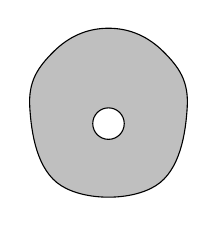
\begin{tikzpicture}
    \draw [fill=gray!50!white] plot [smooth cycle, tension=0.7] coordinates {(0, 1) (-0.7, 0.7) (-1, 0) (-0.6, -1) (0.6, -1) (1, 0) (0.7, 0.7)};
    \draw [fill=white] (0, -0.2113) circle [radius=0.2];
  \end{tikzpicture}
\end{center}
These ``holes'' need not be big holes like this, but just individual points at which a function under consider consideration is singular.

\subsection{Cauchy's theorem}
We now come to the highlight of the course --- Cauchy's theorem. Most of the things we do will be based upon this single important result.

\begin{thm}[Cauchy's theorem]
  If $f(z)$ is analytic in a simply-connected domain $\mathcal{D}$, then for every simple closed contour $\gamma$ in $\mathcal{D}$, we have
  \[
    \oint_\gamma f(z)\;\d z = 0.
  \]
\end{thm}
This is quite a powerful statement, and will allow us to do a lot! On the other hand, this tells us functions that are analytic everywhere are not too interesting. Instead, we will later look at functions like $\frac{1}{z}$ that have singularities.

\begin{proof}(non-examinable)
  The proof of this remarkable theorem is simple (with a catch), and follows from the Cauchy-Riemann equations and Green's theorem. Recall that Green's theorem says
  \[
    \oint_{\partial S} (P \;\d x + Q\;\d y) = \iint_S \left(\frac{\partial Q}{\partial x} - \frac{\partial P}{\partial y}\right)\;\d x\;\d y.
  \]
  Let $u, v$ be the real and imaginary parts of $f$. Then
  \begin{align*}
    \oint_\gamma f(z) \;\d z &= \oint_\gamma (u + iv) (\d x + i\;\d y)\\
    &= \oint_\gamma (u\;\d x - v\;\d y) + i \oint_\gamma (v \;\d x + u \;\d y)\\
    &= \iint_S \left(-\frac{\partial v}{\partial x} - \frac{\partial u}{\partial y}\right)\;\d x\;\d y + i\iint_S \left(\frac{\partial u}{\partial x} - \frac{\partial v}{\partial y}\right)\;\d x \;\d y
  \end{align*}
  But both integrands vanish by the Cauchy-Riemann equations, since $f$ is differentiable throughout $S$. So the result follows.
\end{proof}
Actually, this proof requires $u$ and $v$ to have continuous partial derivatives in $S$, otherwise Green's theorem does not apply. We shall see later that in fact $f$ is differentiable infinitely many time, so actually $u$ and $v$ \emph{do} have continuous partial derivatives. However, our proof of that will utilize Cauchy's theorem! So we are trapped.

Thus a completely different proof (and a very elegant one!) is required if we do not wish to make assumptions about $u$ and $v$. However, we shall not worry about this in this course since it is easy to verify that the functions we use do have continuous partial derivatives. And we are not doing Complex Analysis.

\subsection{Contour deformation}
One useful consequence of Cauchy's theorem is that we can freely deform contours along regions where $f$ is defined without changing the value of the integral.
\begin{prop}
  Suppose that $\gamma_1$ and $\gamma_2$ are contours from $a$ to $b$, and that $f$ is analytic on the contours \emph{and} between the contours. Then
  \[
    \int_{\gamma_1}f(z)\;\d z = \int_{\gamma_2} f(z)\;\d z.
  \]
\end{prop}
\begin{center}
  \begin{tikzpicture}
    \node [circ] {};
    \node [anchor = north east] {$a$};
    \node [circ] at (2, 3) {};
    \node [anchor = south west] at (2, 3) {$b$};

    \draw [->-=0.5] plot [smooth, tension=1] coordinates {(0, 0) (0.5, 2.5) (2, 3)};
    \draw [->-=0.5] plot [smooth, tension=1] coordinates {(0, 0) (1.2, 0.3) (2, 3)};

    \node at (1.8, 0.9) {$\gamma_2$};
    \node at (-0.1, 1.6) {$\gamma_1$};
  \end{tikzpicture}
\end{center}

\begin{proof}
  Suppose first that $\gamma_1$ and $\gamma_2$ do not cross. Then $\gamma_1 - \gamma_2$ is a simple closed contour. So
  \[
    \oint_{\gamma_1 - \gamma_2} f(z)\;\d z = 0
  \]
  by Cauchy's theorem. Then the result follows.

  If $\gamma_1$ and $\gamma_2$ \emph{do} cross, then dissect them at each crossing point, and apply the previous result to each section.
\end{proof}
So we conclude that if $f$ has no singularities, then $\int_a^b f(z)\;\d z$ does not depend on the chosen contour.

This result of path independence, and indeed Cauchy's theorem itself, becomes less surprising if we think of $\int f(z)\;\d z$ as a path integral in $\R^2$, because
\[
  f(z)\;\d z = (u + iv)(\d z + i\;\d y) = (u + iv) \;\d x + (-v + iu)\;\d y
\]
is an exact differential, since
\[
  \pd{y} (u + iv) = \pd{x} (-v + iu)
\]
from the Cauchy-Riemann equations.

The same idea of ``moving the contour'' applies to \emph{closed} contours. Suppose that $\gamma_1$ is a closed contour that can be continuously deformed to another one, $\gamma_2$, inside it; and suppose $f$ has no singularities in the region between them.
\begin{center}
  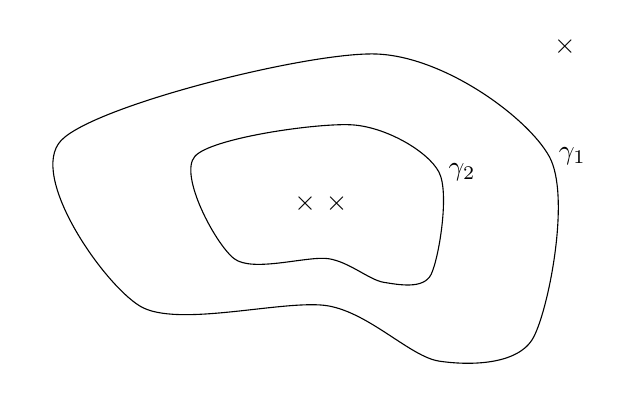
\begin{tikzpicture}
    \draw [->] plot [smooth cycle] coordinates {(-1.2, -0.7) (0, -0.7) (0.7, -1) (1.3, -0.9) (1.4, 0.4) (0.3, 1) (-1.7, 0.6)};
    \draw [->] plot [smooth cycle] coordinates {(-2.4, -1.3) (0, -1.3) (1.4, -2) (2.6, -1.7) (2.8, 0.6) (0.6, 1.9) (-3.4, 0.8)};

    \node [right] at (1.4, 0.4) {$\gamma_2$};
    \node [right] at (2.8, 0.6) {$\gamma_1$};
    \node at (0.1, 0) {$\times$};
    \node at (-0.3, 0) {$\times$};
    \node at (3, 2) {$\times$};
  \end{tikzpicture}
\end{center}
We can instead consider the following contour $\gamma$:
\begin{center}
  \begin{tikzpicture}
    \draw [-<-=0.4, -<-=0.8] plot [smooth cycle] coordinates {(-1.2, -0.7) (0, -0.7) (0.7, -1) (1.3, -0.9) (1.4, 0.4) (0.3, 1) (-1.7, 0.6)};
    \draw [->-=0.3, ->-=0.7, ->-=0.9] plot [smooth cycle] coordinates {(-2.4, -1.3) (0, -1.3) (1.4, -2) (2.6, -1.7) (2.8, 0.6) (0.6, 1.9) (-3.4, 0.8)};

    \node [right] at (2.8, 0.6) {$\gamma$};
    \node at (0.1, 0) {$\times$};
    \node at (-0.3, 0) {$\times$};
    \node at (3, 2) {$\times$};

    \draw [white, very thick] (2.4, 1.07) -- (2.1, 1.3);
    \draw [white, line width=0.5cm] (1.16, 0.65) -- (1.4, 0.4);
    \draw [->-=0.7] (2.4, 1.07) -- (1.4, 0.4);
    \draw [-<-=0.4] (2.1, 1.3) -- (1.16, 0.65);
  \end{tikzpicture}
\end{center}
By Cauchy's theorem, we know $\oint_\gamma f(z)\;\d z = 0$ since $f(z)$ is analytic throughout the region enclosed by $\gamma$. Now we let the distance between the two ``cross-cuts'' tend to zero: those contributions cancel and, in the limit, we have
\[
  \oint_{\gamma_1 - \gamma_2} f(z)\;\d z = 0.
\]
hence we know
\[
  \oint_{\gamma_1} f(z)\;\d z = \oint_{\gamma_2} f(z)\;\d z = 0.
\]

\subsection{Cauchy's integral formula}
\begin{thm}[Cauchy's integral formula]
  Suppose that $f(z)$ is analytic in a domain $\mathcal{D}$ and that $z_0 \in \mathcal{D}$. Then
  \[
    f(z_0) = \frac{1}{2\pi i} \oint_\gamma \frac{f(z)}{z - z_0}\;\d z
  \]
  for any simple closed contour $\gamma$ in $\mathcal{D}$ encircling $z_0$ anticlockwise.
\end{thm}
This result is going to be very important in a brief moment, for proving one thing. Afterwards, it will be mostly useless.

\begin{proof}(non-examinable)
  We let $\gamma_\varepsilon$ be a circle of radius $\varepsilon$ about $z_0$, within $\gamma$.
  \begin{center}
    \begin{tikzpicture}
      \node [circ] {};
      \node [right] {$z_0$};
      \draw [->] circle [radius=0.5];
      \node [right] at (0.5, 0) {$\gamma_\varepsilon$};

      \draw [->] plot [smooth cycle] coordinates {(-2.4, -1.3) (0, -1.3) (1.4, -2) (2.6, -1.7) (2.8, 0.6) (0.6, 1.9) (-3.4, 0.8)};
      \node [right] at (2.8, 0.6) {$\gamma$};
    \end{tikzpicture}
  \end{center}
  Since $\frac{f(z)}{z - z_0}$ is analytic except when $z = z_0$, we know
  \[
    \oint_\gamma \frac{f(z)}{z - z_0} \;\d z = \oint_{\gamma_\varepsilon} \frac{f(z)}{z - z_0}\;\d z.
  \]
  We now evaluate the right integral directly. Substituting $z = z_0 + \varepsilon e^{i\theta}$, we get
  \begin{align*}
    \oint_{\gamma_\varepsilon} \frac{f(z)}{z - z_0}\;\d z &= \int_0^{2\pi} \frac{f(z_0 + \varepsilon e^{i\theta})}{\varepsilon e^{i\theta}} i\varepsilon e^{i\theta} \;\d \theta\\
    &= i\int_0^2\pi (f(z_0) + O(\varepsilon))\;\d \theta\\
    &\rightarrow 2\pi i f(z_0)
  \end{align*}
  as we take the limit $\varepsilon \to 0$. The result then follows.
\end{proof}
So, if we know $f$ on $\gamma$, then we know it at all points within $\gamma$. While this seems magical, it is less surprising if we look at it in another way. We can write $f = u + iv$, where $u$ and $v$ are harmonic functions, i.e.\ they satisfy Laplace's equation. Then if we know the values of $u$ and $v$ on $\gamma$, then what we essentially have is Laplace's equation with Dirichlet boundary conditions! Then the fact that this tells us everything about $f$ within the boundary is just the statement that Laplace's equation with Dirichlet boundary conditions has a unique solution!

The difference between this and what we've got in IA Vector Calculus is that Cauchy's integral formula gives an explicit formula for the value of $f(z_0)$, while in IA Vector Calculus, we just know there is one solution, whatever that might be.

Note that this does not hold if $z_0$ does not lie on or inside $\gamma$, since Cauchy's theorem just gives
\[
  \frac{1}{2\pi i} \oint_\gamma \frac{f(z)}{z - z_0} \;\d z = 0.
\]
Now, we can differentiate Cauchy's integral formula with respect to $z_0$, and obtain
\[
  f'(z_0) = \frac{1}{2\pi i} \oint_\gamma \frac{f(z)}{(z - z_0)^2}\;\d z.
\]
We have just taken the differentiation inside the integral sign. This is valid since \st{it's Complex Methods and we don't care} the integrand, both before and after, is a continuous function of both $z$ and $z_0$.

We see that the integrand is still differentiable. So we can differentiate it again, and obtain
\[
  f^{(n)}(z_0) = \frac{n!}{2\pi i} \oint_{\gamma} \frac{f(z)}{(z - z_0)^{n + 1}}\;\d z.
\]
Hence at any point $z_0$ where $f$ is analytic, \emph{all} its derivatives exist, and we have just found a formula for them. So it is differentiable infinitely many times as advertised.

A classic example of Cauchy's integral formula is Liouville's theorem.
\begin{thm}[Liouville's theorem*]
  Any bounded entire function is a constant.
\end{thm}

\begin{proof}(non-examinable)
  Suppose that $|f(z)| \leq M$ for all $z$, and consider a circle of radius $r$ centered at an arbitrary point $z_0 \in \C$. Then
  \[
    f'(z_0) = \frac{1}{2\pi i} \oint_{|z - z_0| = r} \frac{f(z)}{(z - z_0)^2}\;\d z.
  \]
  Hence we know
  \[
    \frac{1}{2\pi i} \leq \frac{1}{2\pi} \cdot 2\pi r \cdot \frac{M}{r^2} \to 0
  \]
  as $r \to \infty$. So $f'(z_0) = 0$ for all $z_0 \in \C$. So $f$ is constant.
\end{proof}

\section{Laurent series and singularities}
\subsection{Taylor and Laurent series}
If $f$ is analytic at $z_0$, then it has a Taylor series
\[
  f(z) = \sum_{n = 0}^\infty a_n (z - z_0)^n
\]
in a neighbourhood of $z_0$. We will prove this as a special case of the coming proposition. Exactly which neighbourhood it applies in depends on the function. Of course, we know the coefficients are given by
\[
  a_n = \frac{f^{(n)}(z_0)}{n!},
\]
but this doesn't matter. All the standard Taylor series from real analysis apply in $\C$ as well. For example,
\[
  e^z = \sum_{n = 0}^\infty \frac{z^n}{n!},
\]
and this converges for all $z$. Also, we have
\[
  (1 - z)^{-1} = \sum_{n = 0}^\infty z^n.
\]
This converges for $|z| < 1$.

But if $f$ has a singularity at $z_0$, we cannot expect such a Taylor series, since it would imply $f$ is non-singular at $z_0$. However, it turns out we can get a series expansion if we allow ourselves to have negative powers of $z$.

\begin{prop}[Laurent series]
  If $f$ is analytic in an \emph{annulus} $R_1 < |z - z_0| < R_2$, then it has a \emph{Laurent series}
  \[
    f(z) = \sum_{n = -\infty}^\infty a_n (z - z_0)^n.
  \]
  This is convergent within the annulus. Moreover, the convergence is uniform within compact subsets of the annulus.
\end{prop}

\begin{proof}(non-examinable)
  We wlog $z_0 = 0$. Given a $z$ in the annulus, we pick $r_1, r_2$ such that
  \[
    R_1 < r_1 < |z| < r_2 < R_2,
  \]
  and we let $\gamma_1$ and $\gamma_2$ be the contours $|z| = r_1$, $|z| = r_2$ traversed anticlockwise respectively. We choose $\gamma$ to be the contour shown in the diagram below.
  \begin{center}
    \begin{tikzpicture}
      \draw [<-] circle [radius=1];
      \draw [->] circle [radius=2];
      \node [circ] {};
      \node [right] {$z_0$};
      \draw (0, 0) -- (-0.707, 0.707) node [pos=0.5, anchor = south west] {$r_1$};
      \draw (0, 0) -- (-2, 0) node [pos=0.7, above] {$r_2$};

      \node [circ] at (1.3, 0.8) {};
      \node [right] at (1.3, 0.8) {$z$};

      \draw [white, line width=0.5cm] (0.1, 1) -- (-0.1, 1);
      \draw [white, line width=0.5cm] (0.1, 2) -- (-0.1, 2);
      \draw [-<-=0.3] (0.1, 1) -- (0.1, 2);
      \draw [->-=0.6] (-0.1, 1) -- (-0.1, 2);

      \node [right] at (2, 0) {$\gamma$};
    \end{tikzpicture}
  \end{center}
  We now apply Cauchy's integral formula (after a change of notation):
  \[
    f(z) = \frac{1}{2\pi i} \oint_\gamma \frac{f(\zeta)}{\zeta - z} \;\d \zeta.
  \]
  We let the distance between the cross-cuts tend to zero. Then we get
  \[
    f(z) = \frac{1}{2\pi i} \oint_{\gamma_2} \frac{f(\zeta)}{\zeta - z}\;\d z - \frac{1}{2\pi i} \oint_{\gamma_1} \frac{f(\zeta)}{\zeta - z}\;\d \zeta,
  \]
  We have to subtract the second integral because it is traversed in the opposite direction. We do the integrals one by one. We have
  \begin{align*}
    \oint_{\gamma_1} \frac{f(\zeta)}{\zeta - z} &= -\frac{1}{z} \oint_{\gamma_1} \frac{f(\zeta)}{1 - \frac{\zeta}{z}}\;\d \zeta\\
    \intertext{Taking the Taylor series of $\frac{1}{1 - \frac{\zeta}{z}}$, which is valid since $|\zeta| = r_1 < |z|$ on $\gamma_1$, we obtain}
    &= -\frac{1}{z}\oint_{\gamma_1} f(\zeta) \sum_{m = 0}^\infty \left(\frac{\zeta}{z}\right)^m \;\d \zeta\\
    &= -\sum_{m = 0}^\infty z^{-m - 1} \oint_{\gamma_1}f(\zeta) \zeta^m \;\d \zeta.
  \end{align*}
  This is valid since $\oint \sum = \sum \oint$ by uniform convergence. So we can deduce
  \[
    -\frac{1}{2\pi i} \oint_{\gamma_1} \frac{f(\zeta)}{\zeta - z}\;\d \zeta = \sum_{n = -\infty}^{-1} a_n z^n,
  \]
  where
  \[
    a_n = \frac{1}{2\pi i}\oint_{\gamma_1} f(\zeta) \zeta^{-n - 1} \;\d \zeta
  \]
  for $n < 0$.

  Similarly, we obtain
  \[
    \frac{1}{2\pi i} \oint_{\gamma_2} \frac{f(\zeta)}{\zeta - z}\;\d \zeta = \sum_{n = 0}^\infty a_n z^n,
  \]
  for the same definition of $a_n$, except $n \geq 0$, by expanding
  \[
    \frac{1}{\zeta - z} = \frac{1}{\zeta} \frac{1}{1 - \frac{z}{\zeta}} = \sum_{n = 0}^\infty \frac{z^n}{\zeta^{n + 1}}.
  \]
  This is again valid since $|\zeta| = r_2 > |z|$ on $\gamma_2$. Putting these result together, we obtain the Laurent series. The general result then follows by translating the origin by $z_0$.

  We will not prove uniform convergence --- go to IB Complex Analysis.
\end{proof}
It can be shown that Laurent series are unique. Then not only is there a unique Laurent series for each annulus, but if we pick two different annuli on which $f$ is analytic (assuming they overlap), they must have the same coefficient. This is since we can restrict the two series to their common intersection, and then uniqueness requires the coefficients to be must be the same.

Note that the Taylor series is just a special case of Laurent series, and if $f$ is holomorphic at $z_0$, then our explicit formula for the coefficients plus Cauchy's theorem tells us we have $a_n = 0$ for $n < 0$.

Note, however, that we needed the Taylor series of $\frac{1}{1 - z}$ in order to prove Taylor's theorem.

\begin{eg}
  Consider $\frac{e^z}{z^3}$. What is its Laurent series about $z_0 = 0$? We already have a Taylor series for $e^z$, and all we need to do is to divide it by $z^3$. So
  \[
    \frac{e^z}{z^3} = \sum_{n = 0}^\infty \frac{z^{n - 3}}{n!} = \sum_{n = -3}^{\infty} \frac{z^n}{(n + 3)!}.
  \]
\end{eg}

\begin{eg}
  What is the Laurent series for $e^{1/z}$ about $z_0$? Again, we just use the Taylor series for $e^z$. We have
  \[
    e^{\frac{1}{z}} = 1 + \frac{1}{z} + \frac{1}{2! z^2} + \frac{1}{3! z^3} + \cdots.
  \]
  So the coefficients are
  \[
    a_n = \frac{1}{(-n)!}\text{ for }n \leq 0.
  \]
\end{eg}

\begin{eg}
  This is a little bit more tricky. Consider
  \[
    f(z) = \frac{1}{z - a},
  \]
  where $a \in \C$. Then $f$ is analytic in $|z| < |a|$. So it has a Taylor series about $z_0 = 0$ given by
  \[
    \frac{1}{z - a} = -\frac{1}{a}\left(1 - \frac{z}{a}\right)^{-1} = -\sum_{n = 0}^\infty \frac{1}{a^{n + 1}} z^n.
  \]
  What about in $|z| > |a|$? This is an annulus, that goes from $|a|$ to infinity. So it has a Laurent series. We can find it by
  \[
    \frac{1}{z - a} = \frac{1}{z} \left(1 - \frac{a}{z}\right)^{-1} = \sum_{m = 0}^\infty \frac{a^m}{z^{m + 1}} = \sum_{n = -\infty}^{-1} a^{-n - 1} z^n.
  \]
\end{eg}

\begin{eg}
  Now consider
  \[
    f(z) = \frac{e^z}{z^2 - 1}.
  \]
  This has a singularity at $z_0 = 1$ but is analytic in an annulus $0 < |z - z_0| < 2$ (the $2$ comes from the other singularity at $z =-1$). How do we find its Laurent series? This is a standard trick that turns out to be useful --- we write everything in terms of $\zeta = z - z_0$. So
  \begin{align*}
    f(z) &= \frac{e^\zeta e^{z_0}}{\zeta(\zeta + 2)} \\
    &= e^{z_0}{2\zeta} e^{\zeta} \left(1 + \frac{1}{2}\zeta\right)^{-1}\\
    &= \frac{e}{2 \zeta} \left(1 + \zeta + \frac{1}{2!}\zeta^2 + \cdots\right)\left(1 - \frac{1}{2}\zeta + \cdots\right)\\
    &= \frac{e}{2\zeta} \left(1 + \frac{1}{2}\zeta + \cdots\right)\\
    &= \frac{e}{2}\left(\frac{1}{z - z_0} + \frac{1}{2} + \cdots\right).
  \end{align*}
  This is now a Laurent series, with $a_{-1} = \frac{1}{2}e$, $a_0 = \frac{1}{4}e$ etc.
\end{eg}

\begin{eg}
  This doesn't seem to work for $f(z) = z^{-1/2}$. The reason is that the required branch cut of $z^{-\frac{1}{2}}$ would pass through any annulus about $z = 0$. So we cannot find an annulus on which $f$ is analytic.
\end{eg}

The radius of convergence of a Laurent series is at least the size of the annulus, as we that's how we have constructed it. So how large is it?

It turns out the radius of convergence of a Laurent series is always the distance from $z_0$ to the closest singularity of $f(z)$, for we may always choose $R_2$ to be that distance, and obtain a Laurent series valid all the way to $R_2$ (not inclusive). This Laurent series must be the same series as we would have obtained with a smaller radius, because Laurent series are unique.

While this sounds just like some technicalities, this is actually quite useful. When deriving a Laurent series, we can make any assumptions we like about $z - z_0$ being small. Then even if we have derived a Laurent series for a really small neighbourhood, we automatically know the series is valid up to the other point where $f$ is singular.

\subsection{Zeros}
Recall that for a polynomial $p(z)$, we can talk about the \emph{order} of its zero at $z = a$ by looking at the largest power of $(z - a)$ dividing $p$. \emph{A priori}, it is not clear how we can do this for general functions. However, given that everything is a Taylor series, we know how to do this for holomorphic functions.

\begin{defi}[Zeros]
  The \emph{zeros} of an analytic function $f(Z)$ are the points $z_0$ where $f(z_0) = 0$. A zero is of \emph{order $N$} if in its Taylor series $\sum_{n = 0}^\infty a_n (z - z_0)^n$, the first non-zero coefficient is $a_N$.

  Alternatively, it is of order $N$ if $0 = f(z_0) = f'(z_0) = \cdots = f^{(N - 1)}$, but $f^{(N)}(z_0) \not= 0$.
\end{defi}

\begin{defi}[Simple zero]
  A zero of order one is called a \emph{simple zero}.
\end{defi}

\begin{eg}
  $z^3 + iz^2 + z + i = (z - i)(z + i)^2$ has a simple zero at $z = i$ and a zero of order $2$ at $z = -i$.
\end{eg}

\begin{eg}
  $\sinh z$ has zeros where $\frac{1}{2}(e^z - e^{-z}) = 0$, i.e.\ $e^{2z} = 1$, i.e.\ $z = n \pi i$, where $n \in \Z$. The zeros are all simple, since $\cosh n\pi i = \cos n \pi \not= 0$.
\end{eg}

\begin{eg}
  Since $\sinh z$ has a simple zero at $z = \pi i$, we know $\sinh^3 z$ has a zero of order $3$ there. This is since the first term of the Taylor series of $\sinh z$ about $z = \pi i$ has order $1$, and hence the first term of the Taylor series of $\sinh ^3 z$ has order $3$.

  We can also find the Taylor series about $\pi i$ by writing $\zeta = z - \pi i$:
  \begin{align*}
    \sinh^3 z &= [\sinh(\zeta + \pi i)]^3\\
    &= [-\sinh \zeta]^3\\
    &= -\left(\zeta + \frac{1}{3!} + \cdots \right)^3\\
    &= - \zeta^3 - \frac{1}{2} \zeta^5 - \cdots\\
    &= -(z - \pi i)^3 - \frac{1}{2} (z - \pi i)^5 - \cdots.
  \end{align*}
\end{eg}
\subsection{Classification of singularities}
The previous section was rather boring --- you've probably seen all of that before. It is just there as a buildup for our study of singularities. These are in some sense the ``opposites'' of zeros.

\begin{defi}[Isolated singularity]
  Suppose that $f$ has a singularity at $z_0 = z$. If there is a neighbourhood of $z_0$ within which $f$ is analytic, except at $z_0$ itself, then $f$ has an \emph{isolated singularity} at $z_0$. If there is no such neighbourhood, then $f$ has an \emph{essential (non-isolated) singularity} at $z_0$.
\end{defi}

\begin{eg}
  $\cosech z$ has isolated singularities at $z = n \pi i, n \in \Z$, since $\sinh$ has zeroes at these points.
\end{eg}

\begin{eg}
  $\cosech \frac{1}{z}$ has isolated singularities at $z = \frac{1}{n \pi i}$, with $n \not= 0$, and an essential non-isolated singularity at $z = 0$ (since there are other arbitrarily close singularities).
\end{eg}

\begin{eg}
  $\cosech z$ also has an essential non-isolated singularity at $z = \infty$, since $\cosech \frac{1}{z}$ has an essential non-isolated singularity at $z = 0$.
\end{eg}

\begin{eg}
  $\log z$ has a non-isolated singularity at $z = 0$, because it is not analytic at any point on the branch cut. This is normally referred to as a branch point singularity.
\end{eg}

If $f$ has an isolated singularity, at $z_0$, we can find an annulus $0 < |z - z_0| < r$ within which $f$ is analytic, and it therefore has a Laurent series. This gives us a way to classify singularities:

\begin{enumerate}
  \item Check for a branch point singularity.
  \item Check for an essential (non-isolated) singularity.
  \item Otherwise, consider the coefficients of the Laurent series $\sum_{n = -\infty}^\infty a_n (z - z_0)^n$:
    \begin{enumerate}
      \item If $a_n = 0$ for all $n < 0$, then $f$ has a \emph{removable singularity} at $z_0$.
      \item If there is a $N > 0$ such that $a_n = 0$ for all $n < -N$ but $a_{-N} \not= 0$, then $f$ has a \emph{pole} of order $N$ at $z_0$ (for $N = 1, 2, \cdots$, this is also called a \emph{simple pole}, \emph{double pole} etc.).
      \item If there does not exist such an $N$, then $f$ has an \emph{essential isolated singularity}.
    \end{enumerate}
\end{enumerate}
A removable singularity (one with Laurent series $a_0 + a_1 (z - z_0) + \cdots$) is so called because we can remove the singularity by redefining $f(z_0) = a_0 = \lim\limits_{z \to z_0}f(z)$; then $f$ will become analytic at $z_0$.

Let's look at some examples. In fact, we have 10 examples here.
\begin{eg}\leavevmode
  \begin{enumerate}
    \item $\frac{1}{z - i}$ has a simple pole at $z = i$. This is since its Laurent series is, err, $\frac{1}{z - i}$.
    \item $\frac{\cos z}{z}$ has a singularity at the origin. This has Laurent series
      \[
        \frac{\cos z}{z} = z^{-1} - \frac{1}{2}z + \frac{1}{24}z^3 - \cdots,
      \]
      and hence it has a simple pole.
    \item Consider $\frac{z^2}{(z - 1)^3(z - i)^2}$. This has a double pole at $z = i$ and a triple pole at $z = 1$. To show formally that, for instance, there is a double pole at $z = i$, notice first that $\frac{z^2}{(z - 1)^3}$ is analytic at $z = i$. So it has a Taylor series, say,
      \[
        b_0 + b_1(z - i) + b_2(z - i)^2 + \cdots
      \]
      for some $b_n$. Moreover, since $\frac{z^2}{(z - 1)^3}$ is non-zero at $z = i$, we have $b_0 \not= 0$. Hence
      \[
        \frac{z^2}{(z - 1)^3 (z - i)^2} = \frac{b_0}{(z - i)^2} + \frac{b_1}{z - i} + b2 + \cdots.
      \]
      So this has a double pole at $z = i$.
    \item If $g(z)$ has zero of order $N$ at $z = z_0$, then $\frac{1}{g(z)}$ has a pole of order $N$ there, and vice versa. Hence $\cot z$ has a simple pole at the origin, because $\tan z$ has a simple zero there. To prove the general statement, write
      \[
        g(z) = (z - z_0)^N G(z)
      \]
      for some $G$ with $G(z_0) \not= 0$. Then $\frac{1}{G(z)}$ has a Taylor series about $z_0$, and then the result follows.
    \item $z^2$ has a double pole at infinity, since $\frac{1}{\zeta^2}$ has a double pole at $\zeta = 0$.
    \item $e^{1/z}$ has an essential isolated singularity at $z = 0$ because all the $a_n$'s are non-zero for $n \leq 0$.
    \item $\sin \frac{1}{z}$ also has an essential isolated singularity at $z = 0$ because (using the standard Taylor series for $\sin$) there are non-zero $a_n$'s for infinitely many negative $n$.
    \item $f(z) = \frac{e^z - 1}{z}$ has a removable singularity at $z = 0$, because its Laurent series is
      \[
        f(z) = 1 + \frac{1}{2!}z + \frac{1}{3!}z^2 + \cdots.
      \]
      By defining $f(0) = 1$, we would remove the singularity and obtain an entire function.
    \item $f(z) = \frac{\sin z}{z}$ is not defined at $z = 0$, but has a removable singularity there; remove it by setting $f(0) = 1$.
    \item A rational function $f(z) = \frac{P(z)}{Q(z)}$ (where $P, Q$ are polynomials) has a singularity at any point $z_0$ where $Q$ has a zero. Assuming $Q$ has a simple zero, if $P(z_0) = 0$ as well, then the singularity is removable by redefining $f(z_0) = \frac{P'(z_0)}{Q'(z_0)}$ (by L'H\^opital's rule).
  \end{enumerate}
\end{eg}

Near an essential isolated singularity of a function $f(z)$, it can be shown that $f$ takes \emph{all} possible complex values (except at most one) in any neighbourhood, however small. For example, $e^{\frac{1}{z}}$ takes all values except zero. We will not prove this. Even in IB Complex Analysis.

\subsection{Residues}
So far, we've mostly been making lots of definitions. We haven't actually used them to do much useful things. We are almost there. It turns out we can easily evaluate integrals of analytic functions by looking at their Laurent series. Moreover, we don't need the \emph{whole} Laurent series. We just need one of the coefficients.

\begin{defi}[Residue]
  The \emph{residue} of a function $f$ at an isolated singularity $z_0$ is the coefficient $a_{-1}$ in its Laurent expansion about $z_0$. There is no standard notation, but shall denote the residue by $\res\limits_{z = z_0}f(z)$.
\end{defi}

\begin{prop}
  At a \emph{simple} pole, the residue is given by
  \[
    \res_{z = z_0}f(z) = \lim_{z \to z_0} (z - z_0) f(z).
  \]
\end{prop}

\begin{proof}
  We can simply expand the right hand side to obtain
  \begin{align*}
    \lim_{z \to z_0} (z - z_0)\left(\frac{a_{-1}}{z - z_0} + a_0 + a_1(z - z_0) + \cdots\right) &= \lim_{z \to z_0} (a_{-1} + a_0(z - z_0) +\cdots) \\
    &= a_{-1},
  \end{align*}
  as required.
\end{proof}

How about for more complicated poles? More generally, at a pole of order $N$, the formula is a bit messier.
\begin{prop}
  At a pole of order $N$, the residue is given by
  \[
    \lim_{z \to z_0} \frac{1}{(N - 1)!} \frac{\d^{N - 1}}{\d z^{N - 1}} (z - z_0)^N f(z).
  \]
\end{prop}
This can be proved in a similar manner (see example sheet 2).

In practice, a variety of techniques can be used to evaluate residues --- no single technique is optimal for all situations.

\begin{eg}
  Consider $f(z) = \frac{e^z}{z^3}$. We can find the residue by directly computing the Laurent series about $z = 0$:
  \[
    \frac{e^z}{z^3} = z^{-3} + z^{-2} + \frac{1}{2}z^{-1} + \frac{1}{3!} + \cdots.
  \]
  Hence the residue is $\frac{1}{2}$.

  Alternatively, we can use the fact that $f$ has a pole of order $3$ at $z = 0$. So we can use the formula to obtain
  \[
    \res_{z = 0} f(z) = \lim_{z \to 0} \frac{1}{2!} \frac{\d^2}{\d z^2} (z^3 f(z)) = \lim_{z \to 0} \frac{1}{2} \frac{\d^2}{\d z^2} e^z = \frac{1}{2}.
  \]
\end{eg}

\begin{eg}
  Consider
  \[
    g(z) = \frac{e^z}{z^2 - 1}.
  \]
  This has a simple pole at $z = 1$. Recall we have found its Laurent series at $z = 1$ to be
  \[
    \frac{e^z}{z^2 - 1} = \frac{e}{2}\left(\frac{1}{z - 1} + \frac{1}{2} + \cdots\right).
  \]
  So the residue is $\frac{e}{2}$.

  Alternatively, we can use our magic formula to obtain
  \[
    \res_{z = 1} g(z) = \lim_{z \to 1} \frac{(z - 1)e^z}{z^2 - 1} = \lim_{z \to 1}\frac{e^z}{z + 1} = \frac{e}{2}.
  \]
\end{eg}

\begin{eg}
  Consider $h(z) = (z^8 - w^8)^{-1}$, for any complex constant $w$. We know this has $8$ simple poles at $z = w e^{n \pi i/4}$ for $n = 0, \cdots, 7$. What is the residue at $z = w$?

  We can try to compute this directly by
  \begin{align*}
    \res_{z = w} h(z) &= \lim_{z \to w} \frac{z - w}{(z - w)(z - w e^{i \pi /4}) \cdots (z - w e^{7 \pi i/4})}\\
    &= \frac{1}{(w - w e^{i \pi /4}) \cdots (w - w e^{7\pi i/4})}\\
    &= \frac{1}{w^7} \frac{1}{(1 - e^{i\pi/4})\cdots (1 - e^{7 i \pi/4})}
  \end{align*}
  Now we are quite stuck. We don't know what to do with this. We can think really hard about complex numbers and figure out what it should be, but this is difficult. What we should do is to apply L'H\^opital's rule and obtain
  \[
    \res_{z = w}h(z) = \lim_{z \to w} \frac{z - w}{z^8 - w^8} = \frac{1}{8z^7} = \frac{1}{8w^7}.
  \]
\end{eg}

\begin{eg}
  Consider the function $(\sinh \pi z)^{-1}$. This has a simple pole at $z = ni$ for all integers $n$ (because the zeros of $\sinh z$ are at $n\pi i$ and are simple). Again, we can compute this by finding the Laurent expansion. However, it turns out it is easier to use our magic formula together with L'H\^opital's rule. We have
  \[
    \lim_{z \to ni} \frac{z - ni}{\sinh \pi z} = \lim_{z \to ni} \frac{1}{\pi \cosh \pi z} = \frac{1}{\pi \cosh n\pi i} = \frac{1}{\pi \cos n\pi} = \frac{(-1)^n}{\pi}.
  \]
\end{eg}

\begin{eg}
  Consider the function $(\sinh^3 z)^{-1}$. This time, we find the residue by looking at the Laurent series. We first look at $\sinh^3 z$. This has a zero of order $3$ at $z = \pi i$. Its Taylor series is
  \[
    \sinh^3 z = -(z - \pi i)^3 - \frac{1}{2}(z - \pi i)^5.
  \]
  Therefore
  \begin{align*}
    \frac{1}{\sinh^3 z} &= -(z - \pi i)^{-3} \left(1 + \frac{1}{2}(z - \pi i)^2 + \cdots\right)^{-1}\\
    &= -(z - \pi i)^{-3}\left(1 - \frac{1}{2}(z - \pi i)^2 + \cdots\right)\\
    &= -(z - \pi i)^{-3} + \frac{1}{2}(z - \pi i)^{-1} + \cdots
  \end{align*}
  Therefore the residue is $\frac{1}{2}$.
\end{eg}
So we can compute residues. But this seems a bit odd --- why are we interested in the coefficient of $a_{-1}$? Out of the doubly infinite set of coefficients, why $a_{-1}$?

The purpose of this definition is to aid in evaluating integrals $\oint f(z)\;\d z$, where $f$ is a function analytic within the anticlockwise simple closed contour $\gamma$, except for an isolated singularity $z_0$. We let $\gamma_r$ be a circle of radius $r$ centered on $z_0$, lying within $\gamma$.
\begin{center}
  \begin{tikzpicture}
    \draw [->] plot [smooth cycle] coordinates {(-1.2, -0.7) (0, -0.7) (0.7, -1) (1.3, -0.9) (1.4, 0.4) (0.3, 1) (-1.7, 0.6)};
    \node [circ] at (0, 0) {};
    \node [right] at (0, 0) {$z_0$};
    \draw [->] circle [radius=0.5];
    \node [right] at (0.5, 0) {$\gamma_r$};
  \end{tikzpicture}
\end{center}
Now $f$ has some Laurent series expansion $\sum_{n = -\infty}^\infty a_n (z - z_0)^n$ about $z_0$. Recall that we are allowed to deform contours along regions where $f$ is analytic. So
\begin{align*}
  \oint_\gamma f(z)\;\d z &= \oint_{\gamma_r} f(z)\;\d z\\
  &= \oint_{\gamma_r} \sum_{n = -\infty}^\infty a_n (z - z_0)^n \;\d z\\
  \intertext{By uniform convergence, we can swap the integral and sum to obtain}
  &= \sum_{n = -\infty}^\infty a_n \oint_{\gamma_r} (z - z_0)^n \;\d z
\end{align*}
We know how to integrate around the circle:
\begin{align*}
  \oint_{\gamma_r}(z - z_0)^n \;\d z &= \int_0^{2\pi} r^n e^{in \theta} i r e^{i \theta}\;\d \theta\\
  &= ir^{n + 1} \int_0^{2\pi} e^{i(n + 1)\theta}\;\d \theta\\
  &=
  \begin{cases}
    2 \pi i & n = -1\\
    \frac{r^{n + 1}}{n + 1}\left[ e^{i(n + 1)\theta}\right] = 0, &n \not= -1
  \end{cases}.
\end{align*}
Hence we have
\[
  \oint_\gamma f(z)\;\d z = 2\pi i a_{-1} = 2 \pi i \res_{z = z_0}f(z).
\]
\begin{thm}
  $\gamma$ be an anticlockwise simple closed contour, and let $f$ be analytic within $\gamma$ except for an isolated singularity $z_0$. Then
  \[
    \oint_\gamma f(z)\;\d z = 2\pi i a_{-1} = 2 \pi i \res_{z = z_0}f(z).
  \]
\end{thm}

\section{The calculus of residues}
Nowadays, we use ``calculus'' to mean differentiation and integration. However, historically, the word ``calculus'' just means doing calculations. The word ``calculus'' in the calculus of residues does not refer to differentiation and integration, even though in this case they \emph{are} related, but this is just a coincidence.

\subsection{The residue theorem}
We are now going to massively generalize the last result we had in the previous chapter. We are going consider a function $f$ with \emph{many} singularities, and obtain an analogous formula.

\begin{thm}[Residue theorem]
  Suppose $f$ is analytic in a simply-connected region except at a finite number of isolated singularities $z_1, \cdots, z_n$, and that a simple closed contour $\gamma$ encircles the singularities anticlockwise. Then
  \[
    \oint_\gamma f(z)\;\d z = 2\pi i \sum_{k = 1}^n \res_{z = z_k} f(z).
  \]
\end{thm}
\begin{center}
  \begin{tikzpicture}
    \draw [->-=0.3, ->-=0.7, ->-=0.9] plot [smooth cycle] coordinates {(-2.4, -1.3) (0, -1.3) (1.4, -2) (2.6, -1.7) (2.8, 0.6) (0.6, 1.9) (-3.4, 0.8)};
    \node [circ] (z1) at (1.8, 0) {};
    \node [right] at (z1) {$z_1$};
    \node [circ] (z2) at (0, 1) {};
    \node [right] at (z2) {$z_2$};
    \node [circ] (z3) at (-2, -0.5) {};
    \node [right] at (z3) {$z_3$};
    \node at (3, 1) {$\gamma$};
  \end{tikzpicture}
\end{center}
Note that we have already proved the case $n = 1$ in the previous section. To prove this, we just need a difficult drawing.

\begin{proof}
  Consider the following curve $\hat{\gamma}$, consisting of small clockwise circles $\gamma_1, \cdots, \gamma_n$ around each singularity; cross cuts, which cancel in the limit as they approach each other, in pairs; and the large outer curve (which is the same as $\gamma$ in the limit).
  \begin{center}
    \begin{tikzpicture}
      \draw [->-=0.3, ->-=0.7, ->-=0.9] plot [smooth cycle] coordinates {(-2.4, -1.3) (0, -1.3) (1.4, -2) (2.6, -1.7) (2.8, 0.6) (0.6, 1.9) (-3.4, 0.8)};
      \node [circ] (z1) at (1.8, 0) {};
      \node [circ] (z2) at (0, 1) {};
      \node [circ] (z3) at (-2, -0.5) {};

      \node at (3, 1) {$\hat{\gamma}$};
      \draw [-<-=0.5] (z1) circle [radius=0.5];
      \draw [-<-=0.75](z2) circle [radius=0.5];
      \draw [<-] (z3) circle [radius=0.5];

      \draw [white, line width=0.5cm] (2.91, 0.1) -- (2.92, -0.1);
      \draw [white, line width=0.5cm] (2.29, 0.1) -- (2.29, -0.1);
      \draw (2.29, 0.1) -- (2.91, 0.1);
      \draw (2.29, -0.1) -- (2.92, -0.1);

      \draw [white, line width=0.5cm] (0.1, 1.49) -- (-0.1, 1.49);
      \draw [white, line width=0.5cm] (0.1, 1.86) -- (-0.1, 1.84);
      \draw (0.1, 1.49) -- (0.1, 1.86);
      \draw (-0.1, 1.49) -- (-0.1, 1.84);

      \draw [white, line width=0.5cm] (-3.05, -0.6) -- (-3.18, -0.4);
      \draw [white, line width=0.5cm] (-2.49, -0.6) -- (-2.49, -0.4);
      \draw (-2.49, -0.6) -- (-3.05, -0.6);
      \draw (-2.49, -0.4) -- (-3.18, -0.4);

      \node [right] at (z1) {$z_1$};
      \node [right] at (z2) {$z_2$};
      \node [right] at (z3) {$z_3$};
    \end{tikzpicture}
  \end{center}
  Note that $\hat{\gamma}$ encircles no singularities. So $\oint_{\hat{\gamma}}f(z)\;\d z = 0$ by Cauchy's theorem. So in the limit when the cross cuts cancel, we have
  \[
    \oint_\gamma f(z)\;\d z + \sum_{k = 1}^n \oint_{\gamma_k} f(z)\;\d z = \oint_{\hat{\gamma}} f(z)\;\d z = 0.
  \]
  But from what we did in the previous section, we know
  \[
    \oint_{\gamma_k}f(z)\;\d z = -2\pi i \res_{z = z_k} f(z),
  \]
  since $\gamma_k$ encircles only one singularity, and we get a negative sign since $\gamma_k$ is a clockwise contour. Then the result follows.
\end{proof}

This is the key practical result of this course. We are going to be using this very extensively to compute integrals.

\subsection{Applications of the residue theorem}
We now use the residue theorem to evaluate lots of real integrals.
\begin{eg}
  We shall evaluate
  \[
    I = \int_0^\infty \frac{\d x}{1 + x^2},
  \]
  which we can already do so by trigonometric substitution. While it is silly to integrate this with the residue theorem here, since integrating directly is much easier, this technique is a much more general method, and can be used to integrate many other things. On the other hand, our standard tricks easily become useless when we change the integrand a bit, and we need to find a completely different method.

  Consider
  \[
    \oint_\gamma \frac{\d z}{1 + z^2},
  \]
  where $\gamma$ is the contour shown: from $-R$ to $R$ along the real axis ($\gamma_0$), then returning to $-R$ via a semicircle of radius $R$ in the upper half plane ($\gamma_R$). This is known as ``closing in the upper-half plane''.
  \begin{center}
    \begin{tikzpicture}
      \draw [->] (-3, 0) -- (3, 0);
      \draw [->] (0, -1) -- (0, 3);

      \draw [mred, thick, ->-=0.3, ->-=0.8] (-2, 0) -- (2, 0) node [pos=0.3, below] {$\gamma_0$} arc(0:180:2) node [pos=0.3, right] {$\gamma_R$};

      \node [below] at (-2, 0) {$-R$};
      \node [below] at (2, 0) {$R$};

      \node at (0, 1) {$\times$};
      \node [right] at (0, 1) {$i$};
    \end{tikzpicture}
  \end{center}
  Now we have
  \[
    \frac{1}{1 + z^2} = \frac{1}{(z + i)(z - i)}.
  \]
  So the only singularity enclosed by $\gamma$ is a simple pole at $z = i$, where the residue is
  \[
    \lim_{z \to i} \frac{1}{z + i} = \frac{1}{2i}.
  \]
  Hence
  \[
    \int_{\gamma_0} \frac{\d z}{1 + z^2} + \int_{\gamma_R} \frac{\d z}{1 + z^2} = \int_\gamma \frac{\d z}{1 + z^2}= 2\pi i \cdot \frac{1}{2i} = \pi.
  \]
  Let's now look at the terms individually. We know
  \[
    \int_{\gamma_0} \frac{\d z}{1 + z^2} = \int_{-R}^R \frac{\d x}{1 + x^2} \to 2I
  \]
  as $R \to \infty$. Also,
  \[
    \int_{\gamma_R} \frac{\d z}{1 + z^2} \to 0
  \]
  as $R \to \infty$ (see below). So we obtain in the limit
  \[
    2I + 0 = \pi.
  \]
  So
  \[
    I = \frac{\pi}{2}.
  \]
  Finally, we need to show that the integral about $\gamma_R$ vanishes as $R \to \infty$. This is usually a bit tricky. We can use a formal or informal argument. We first do it formally: by the triangle inequality, we know
  \[
    |1 + z^2| \geq |1 - |z|^2|.
  \]
  On $\gamma_R$, we know $|z| = R$. So for large $R$, we get
  \[
    |1 + z^2| \geq 1 - R^2 = R^2 - 1.
  \]
  Hence
  \[
    \frac{1}{|1 + z^2|} \leq \frac{1}{R^2 - 1}.
  \]
  Thus we can bound the integral by
  \[
    \left|\int_{\gamma_R} \frac{\d z}{1 + z^2}\right| \leq \pi R \cdot \frac{1}{R^2 - 1} \to 0
  \]
  as $R \to \infty$.

  We can also do this informally, by writing
  \[
    \left|\int_{\gamma_R} \frac{\d z}{1 + z^2}\right| \leq \pi R \sup_{z \in \gamma_R} \left|\frac{1}{1 + z^2}\right| = \pi R \cdot O(R^{-2}) = O(R^{-1}) \to 0.
  \]
\end{eg}
This example is not in itself impressive, but the method adapts easily to more difficult integrals. For example, the same argument would allow us to integrate $\frac{1}{1 + x^8}$ with ease.

Note that we could have ``closed in the lower half-plane'' instead.
\begin{center}
  \begin{tikzpicture}
    \draw [->] (-3, 0) -- (3, 0);
    \draw [->] (0, -3) -- (0, 1);

    \draw [mred, thick, ->-=0.3, ->-=0.8] (-2, 0) -- (2, 0) arc(0:-180:2);

    \node [above] at (-2, 0) {$-R$};
    \node [above] at (2, 0) {$R$};

    \node at (0, -1) {$\times$};
    \node [left] at (0, -1) {$-i$};
  \end{tikzpicture}
\end{center}
Most of the argument would be unchanged; the residue would now be
\[
  \res_{z = -i} \frac{1}{1 + z^2} = -\frac{1}{2i},
\]
but the contour is now traversed clockwise. So we collect another minus sign, and obtain the same result.

Let's do more examples.
\begin{eg}
  To find the integral
  \[
    I = \int_0^\infty \frac{\d x}{(x^2 + a^2)^2},
  \]
  where $a > 0$ is a real constant, consider the contour integral
  \[
    \int_{\gamma} \frac{\d z}{(z^2 + a^2)^2},
  \]
  where $\gamma$ is exactly as above. The only singularity within $\gamma$ is a pole of order $2$ at $z = ia$, at which the residue is
  \begin{align*}
    \lim_{z \to ia} \frac{\d}{\d z} \frac{1}{(z + ia)^2} &= \lim_{z \to ia} \frac{-2}{(z + ia)^3} \\
    &= \frac{-2}{-8ia^3} \\
    &=-\frac{1}{4}ia^{-3}.
  \end{align*}
  We also have to do the integral around $\gamma_R$. This still vanishes as $R \to \infty$, since
  \[
    \left|\int_{\gamma_R} \frac{\d z}{(z^2 + a^2)^2}\right| \leq \pi R \cdot O(R^{-4}) = O(R^{-3}) \to 0.
  \]
  Therefore
  \[
    2I = 2\pi i \left(-\frac{1}{4}ia^{-3}\right).
  \]
  So
  \[
    I = \frac{\pi}{4a^3}.
  \]
\end{eg}

\begin{eg}
  Consider
  \[
    I = \int_0^\infty \frac{\d x}{1 + x^4}.
  \]
  We use the same contour again. There are simple poles of $\frac{1}{1 + z^4}$ at
  \[
    e^{\pi i/4}, e^{3\pi i/4}, e^{-\pi i/4}, e^{-3\pi i/4},
  \]
  but only the first two are enclosed by the contour.
  \begin{center}
    \begin{tikzpicture}
      \draw [->] (-3, 0) -- (3, 0);
      \draw [->] (0, -1) -- (0, 3);

      \draw [mred, thick, ->-=0.3, ->-=0.8] (-2, 0) -- (2, 0) node [pos=0.3, below] {$\gamma_0$} arc(0:180:2) node [pos=0.3, right] {$\gamma_R$};

      \node [below] at (-2, 0) {$-R$};
      \node [below] at (2, 0) {$R$};

      \node at (1, 1) {$\times$};
      \node at (-1, 1) {$\times$};
    \end{tikzpicture}
  \end{center}
  The residues at these two poles are $-\frac{1}{4}e^{\pi i/4}$ and $+\frac{1}{4} e^{-\pi i/4}$ respectively. Hence
  \[
    2 I = 2\pi i \left(-\frac{1}{4}e^{\pi i/4} + \frac{1}{4} e^{-\pi i/4}\right).
  \]
  Working out some algebra, we find
  \[
    I = \frac{\pi}{2\sqrt{2}}.
  \]
\end{eg}

\begin{eg}
  There is another way of doing the previous integral. Instead, we use this quarter-circle as shown:
  \begin{center}
    \begin{tikzpicture}
      \draw [->] (-1, 0) -- (3, 0);
      \draw [->] (0, -1) -- (0, 3);

      \draw [mred, thick, ->-=0.2, ->-=0.5, ->-=0.9] (0, 0) -- (2, 0) node [pos=0.5, below] {$\gamma_0$} arc(0:90:2) node [pos=0.5, right] {$\gamma_1$} -- (0, 0) node [pos=0.5, left] {$\gamma_2$};

      \node [left] at (0, 2) {$iR$};
      \node [below] at (2, 0) {$R$};

      \node at (1, 1) {$\times$};
    \end{tikzpicture}
  \end{center}
  In words, $\gamma$ consists of the real axis from $0$ to $R$ ($\gamma_0$); the arc circle from $R$ to $iR$ ($\gamma_1$); and the imaginary axis from $iR$ to $0$ ($\gamma_2$).

  Now
  \[
    \int_{\gamma_0}\frac{\d z}{1 + z^4} \to I\text{ as }R \to \infty,
  \]
  and along $\gamma_2$ we substitute $z = iy$ to obtain
  \[
    \int_{\gamma_0} \frac{\d z}{1 + z^4} = \int_R^0 i\frac{\d y}{1 + y^4} \to -i I\text{ as }R \to \infty.
  \]
  Finally, the integral over $\gamma_1$ vanishes as before. We enclose only one pole, which makes the calculation a bit easier than what we did last time. In the limit, we get
  \[
    I - iI = 2\pi i \left(-\frac{1}{4} e^{\pi i/4}\right),
  \]
  and we again obtain
  \[
    I = \frac{\pi}{2 \sqrt{2}}.
  \]
\end{eg}

\begin{eg}
  We now look at trigonometric integrals of the form :
  \[
    \int_0^{2\pi} f(\sin \theta, \cos \theta)\;\d \theta.
  \]
  We substitute
  \[
    z = e^{i\theta},\quad \cos \theta = \frac{1}{2}(z + z^{-1}),\quad \sin \theta = \frac{1}{2i}(z - z^{-1}).
  \]
  We then end up with a closed contour integral.

  For example, consider the integral
  \[
    I = \int_0^{2\pi}\frac{\d \theta}{a + \cos \theta},
  \]
  where $a > 1$. We substitute $z = e^{i\theta}$, so that $\d z = iz\;\d \theta$ and $\cos \theta = \frac{1}{2}(z + z^{-1})$. As $\theta$ increases from $1$ to $2\pi$, $z$ moves round the circle $\gamma$ of radius $1$ in the complex plane. Hence
  \[
    I = \oint_{\gamma} \frac{(iz)^{-1}\;\d z}{a + \frac{1}{2}(z + z^{-1})} = -2i \oint_{\gamma} \frac{\d z}{z^2 + 2az + 1}.
  \]
  \begin{center}
    \begin{tikzpicture}
      \draw [->] (-3, 0) -- (3, 0);
      \draw [->] (0, -3) -- (0, 3);
      \draw [mred, thick, ->-=0.2] circle [radius=1.8];
      \node [right] at (1.2726, 1.2726) {$\gamma$};

      \node (z-) at (-2.5, 0) {$\times$};
      \node [below] at (z-) {$z_-$};

      \node (z+) at (-1.2, 0) {$\times$};
      \node [below] at (z+) {$z_+$};
    \end{tikzpicture}
  \end{center}
  We now solve the quadratic to obtain the poles, which happen to be
  \[
    z_{\pm} = -a \pm \sqrt{a^2 - 1}.
  \]
  With some careful thinking, we realize $z_+$ is inside the circle, while $z_-$ is outside.

  To find the residue, we notice the integrand is equal to
  \[
    \frac{1}{(z - z_+)(z - z_-)}.
  \]
  So the residue at $z = z_+$ is
  \[
    \frac{1}{z_+ - z_-} = \frac{1}{2\sqrt{a^2 - 1}}.
  \]
  Hence
  \[
    I = -2i\left(\frac{2\pi i}{2\sqrt{a^2 - 1}}\right) = \frac{2\pi}{\sqrt{a^2 - 1}}.
  \]
\end{eg}

\begin{eg}
  Integrating a function with a branch cut is a bit more tricky, and requires a ``keyhole contour''. Suppose we want to integrate
  \[
    I = \int_0^\infty \frac{x^\alpha}{1 + \sqrt{2}x + x^2}\;\d x,
  \]
  with $-1 < \alpha < 1$ so that the integral converges. We need a branch cut for $z^{\alpha}$. We take our branch cut to be along the positive real axis, and define
  \[
    z^\alpha = r^\alpha e^{i\alpha \theta},
  \]
  where $z = re^{i\theta}$ and $0 \leq \theta < 2\pi$. We use the following keyhole contour:
  \begin{center}
    \begin{tikzpicture}
      \draw [->] (-3, 0) -- (3, 0);
      \draw [->] (0, -3) -- (0, 3);
      \draw [thick,decorate, decoration=zigzag] (0, 0) -- (3, 0);

      \draw [mred, thick, ->-=0.1, ->-=0.45, ->-=0.75, ->-=0.84, ->-=0.95] (1.977, 0.3) arc(8.63:351.37:2) node [pos=0.15, anchor = south west] {$C_R$} -- (0.4, -0.3) arc(323.13:36.87:0.5) node [pos=0.7, left] {$C_\varepsilon$} -- cycle;

      \node [circ] at (0, 0) {};

      \node at (-1, -1) {$\times$};
      \node [right] at (-1, -1) {$e^{5\pi i/4}$};
      \node at (-1, 1) {$\times$};
      \node [right] at (-1, 1) {$e^{3\pi i/4}$};
    \end{tikzpicture}
  \end{center}
  This consists of a large circle $C_R$ of radius $R$, a small circle $C_\varepsilon$ of radius $\varepsilon$, and the two lines just above and below the branch cut. The idea is to simultaneously take the limit $\varepsilon \to 0$ and $R \to \infty$.

  We have four integrals to work out. The first is
  \[
    \int_{\gamma_R} \frac{z^\alpha}{1 + \sqrt{2}z + z^2} \;\d z= O(R^{\alpha - 2}) \cdot 2\pi R = O(R^{\alpha - 1}) \to 0
  \]
  as $R \to \infty$. To obtain the contribution from $\gamma_\varepsilon$, we substitute $z = \varepsilon e^{i\theta}$, and obtain
  \[
    \int_{2\pi}^0 \frac{\varepsilon^\alpha e^{i\alpha\theta}}{1 + \sqrt{2} \varepsilon e^{i\theta} + \varepsilon^2 e^{2i \theta}} i \varepsilon e^{i\theta}\;\d \theta = O(\varepsilon^{\alpha + 1}) \to 0.
  \]
  Finally, we look at the integrals above and below the branch cut. The contribution from just above the branch cut is
  \[
    \int_\varepsilon^R \frac{x^{\alpha}}{1 + \sqrt{2}x + x^2}\;\d x \to I.
  \]
  Similarly, the integral below is
  \[
    \int_R^\varepsilon \frac{x^\alpha e^{2\alpha \pi i}}{1 + \sqrt{2}x + x^2} \to -e^{2\alpha \pi i}I.
  \]
  So we get
  \[
    \oint_\gamma \frac{z^\alpha}{1 + \sqrt{2} z + z^2}\;\d z \to (1 - e^{2\alpha \pi i})I.
  \]
  All that remains is to compute the residues. We write the integrand as
  \[
    \frac{z^\alpha}{(z - e^{3e\pi i/4})(z - e^{5\pi i/4})}.
  \]
  So the poles are at $z_0 = e^{3\pi i/4}$ and $z_1 = e^{5\pi i/4}$. The residues are
  \[
    \frac{e^{3\alpha \pi i/4}}{\sqrt{2} i},\quad \frac{e^{5\alpha\pi i/4}}{-\sqrt{2}i}
  \]
  respectively. Hence we know
  \[
    (1 - e^{2\alpha \pi i})I = 2\pi i\left(\frac{e^{3\alpha \pi i/4}}{\sqrt{2} i} + \frac{e^{5\alpha \pi i/4}}{-\sqrt{2} i}\right).
  \]
  In other words, we get
  \[
    e^{\alpha \pi i}(e^{-\alpha \pi i} - e^{\alpha \pi i})I = \sqrt{2} \pi e^{\alpha \pi i} (e^{-\alpha \pi i/4} - e^{\alpha \pi i/4}).
  \]
  Thus we have
  \[
    I = \sqrt{2} \pi \frac{\sin(\alpha \pi/4)}{\sin (\alpha\pi)}.
  \]
  Note that we we labeled the poles as $e^{3\pi i/4}$ and $e^{5 \pi i/4}$. The second point is the same point as $e^{-3\pi i/4}$, but it would be wrong to label it like that. We have decided at the beginning to pick the branch such that $0 \leq \theta < 2\pi$, and $-3\pi i/4$ is \emph{not} in that range. If we wrote it as $e^{-3\pi i/4}$ instead, we might have got the residue as $e^{-3 \alpha \pi i/4}/(-\sqrt{2}i)$, which is not the same as $e^{5 \alpha \pi i/4}/(-\sqrt{2}i)$.
\end{eg}
Note that the need of a branch cut does \emph{not} mean we must use a keyhole contour. Sometimes, we can get away with the branch cut and contour chosen as follows:
\begin{center}
  \begin{tikzpicture}
    \draw [->] (-3, 0) -- (3, 0);
    \draw [->] (0, -3) -- (0, 3);
    \draw [thick, decorate, decoration=zigzag] (0, 0) -- (0, -3);

    \node [circ] at (0, 0) {};

    \draw [mred, thick, ->-=0.1, ->-=0.4, ->-=0.7] (-2, 0) node [below] {$-R$} -- (-0.4, 0) node [below] {$\varepsilon$} arc(180:0:0.4) node [below] {$\varepsilon$} -- (2, 0) node [below] {$R$} arc(0:180:2);

    \node at (0, 1) {$\times$};
    \node [right] at (0, 1) {$i$};
  \end{tikzpicture}
\end{center}

\subsection{Further applications of the residue theorem using rectangular contours}
\begin{eg}
  We want to calculate
  \[
    I = \int_{-\infty}^\infty \frac{e^{\alpha x}}{\cosh x}\;\d x,
  \]
  where $\alpha \in (-1, 1)$. We notice this has singularities at $x = \left(n + \frac{1}{2}\right)\pi i$ for all $n$. So if we used our good, old semi-circular contours, then we would run into infinitely many singularities as $R \to \infty$.

  Instead, we abuse the periodic nature of $\cosh$, and consider the following rectangular contour:
  \begin{center}
    \begin{tikzpicture}
      \draw [->] (-3, 0) -- (3, 0);
      \draw [->] (0, -1) -- (0, 3);

      \draw [mred, thick, ->-=0.3, ->-=0.78] (-2, 0) node [below] {$-R$} -- (2, 0) node [pos=0.7, below] {$\gamma_0$} node [below] {$R$} -- (2, 1.5) node [pos=0.5, right] {$\gamma_R^+$} -- (-2, 1.5) node [pos=0.3, above] {$\gamma_1$} -- (-2, 0) node [pos=0.5, left] {$\gamma_R^-$};

      \node at (0, 0.75) {$\times$};
      \node [left] at (0, 0.75) {$\frac{\pi i}{2}$};

      \node [circ] at (0, 1.5) {};
      \node [anchor = south east] at (0, 1.5) {$\pi i$};
    \end{tikzpicture}
  \end{center}
  We see that
  \[
    \int_{\gamma_0} \frac{e^{\alpha z}}{\cosh z} \;\d z\to I \text{ as }R \to \infty.
  \]
  Also,
  \begin{align*}
    \int_{\gamma_1} \frac{e^{\alpha z}}{\cosh z} \;\d z &= \int_R^{-R} \frac{e^{\alpha(x + \pi i)}}{\cosh(x + \pi i)}\;\d x\\
    &= e^{\alpha \pi i} \int_R^{-R} \frac{e^{\alpha x}}{-\cosh x}\;\d x\\
    &\to e^{\alpha \pi i}I.
  \end{align*}
  On the $\gamma_R^+$, we have
  \[
    \cosh z = \cosh(R + iy) = \cosh R \cos y + i\sinh R \sin y.
  \]
  So
  \[
    |\cosh z| = \sqrt{\cosh^2 R \cos^2 y + \sinh^2 R \sin^2 y}.
  \]
  We now use the formula $\cosh^2 R = 1 + \sinh^2 R$, and magically obtain
  \[
    |\cosh z| = \sqrt{\cos^2 y + \sinh^2 R} \geq \sinh R.
  \]
  Hence
  \[
    \left|\frac{e^{\alpha z}}{\cosh z}\right| \leq \frac{|e^{\alpha R}e^{\alpha i y}|}{\sinh R} = \frac{e^{\alpha R}}{\sinh R} = O(e^{(\alpha - 1)R}) \to 0.
  \]
  Hence as $R \to \infty$,
  \[
    \int_{\gamma^+} \frac{e^{\alpha z}}{\cosh z} \;\d z\to 0.
  \]
  Similarly, the integral along $\gamma^-$ vanishes.

  Finally, we need to find the residue. The only singularity inside the contour is at $\frac{\pi i}{2}$, where the residue is
  \[
    \frac{e^{\alpha \pi i/2}}{\sinh \frac{\pi i}{2}} = -ie^{\alpha \pi i/2}.
  \]
  Hence we get
  \[
    I ( 1 + e^{\alpha \pi i}) = 2\pi i (-i e^{\alpha \pi i/2}) = 2\pi ie^{\alpha \pi i/2}.
  \]
  So we find
  \[
    I = \frac{\pi}{\cos(\alpha \pi/2)}.
  \]
\end{eg}
These rectangular contours tend to be useful for trigonometric and hyperbolic functions.

\begin{eg}
  Consider the integral
  \[
    \int_\gamma \frac{\cot \pi z}{z^2}\;\d z,
  \]
  where $\gamma$ is the square contour shown with corners at $(N + \frac{1}{2})(\pm 1 \pm i)$, where $N$ is a large integer, avoiding the singularities
  \begin{center}
    \begin{tikzpicture}
      \draw [->] (-3, 0) -- (3, 0);
      \draw [->] (0, -3) -- (0, 3);

      \foreach \x in {-2.5,-2,...,2.5} {
        \node at (\x, 0) {$\times$};
      }

      \draw [mred, thick] (1.75, 1.75) rectangle (-1.75, -1.75);

      \node [anchor = south west] at (0, 1.75) {$(N + \frac{1}{2})i$};
      \node [anchor = north west] at (0, -1.75) {$-(N + \frac{1}{2})i$};
      \node [anchor = south west] at (1.75, 0) {$N + \frac{1}{2}$};
      \node [anchor = south east] at (-1.75, 0) {$-(N + \frac{1}{2})$};

      \node [circ] at (0, 1.75) {};
      \node [circ] at (0, -1.75) {};
      \node [circ] at (1.75, 0) {};
      \node [circ] at (-1.75, 0) {};
    \end{tikzpicture}
  \end{center}
  There are simple poles at $z = n\in \Z\setminus \{0\}$, with residues $\frac{1}{n^2 \pi}$, and a triple pole at $z = 0$ with residue $-\frac{1}{3}\pi$ (from the Taylor series for $z^2 \tan \pi z$). It turns out the integrals along the sides all vanish as $N \to \infty$ (see later). So we know
  \[
    2\pi i\left(2 \sum_{n = 1}^N \frac{1}{n^2} \pi - \frac{\pi}{3}\right) \to 0
  \]
  as $N \to \infty$. In other words,
  \[
    \sum_{n = 1}^N \frac{1}{n^2} = \frac{\pi^2}{6}.
  \]
  This is probably the most complicated and most inefficient way of computing this series. However, notice we can easily modify this to fund the sum of $\frac{1}{n^3}$, or $\frac{1}{n^4}$, or any complicated sum we can think of.

  Hence all that remains is to show that the integrals along the sides vanish. On the right-hand side, we can write $z = N + \frac{1}{2} + iy$. Then
  \[
    |\cot \pi z| = \left|\cot\left( \left(N + \frac{1}{2}\right) + i \pi y\right)\right| = |-\tan i \pi y| = |\tanh \pi y| \leq 1.
  \]
  So $\cot \pi z$ is bounded on the vertical side. Since we are integrating $\frac{\cot \pi z}{z^2}$, the integral vanishes as $N \to \infty$.

  Along the top, we get $z = x + \left(N + \frac{1}{2}\right)i$. This gives
  \[
    |\cot \pi z| = \frac{\sqrt{\cosh^2 \left(N + \frac{1}{2}\right) \pi - \sin^2 \pi x}}{\sqrt{\sinh^2 \left(N + \frac{1}{2}\right)\pi + \sin^2 \pi x}} \leq \coth\left(N + \frac{1}{2}\right) \pi \leq \coth \frac{\pi}{2}.
  \]
  So again $\cot \pi z$ is bounded on the top side. So again, the integral vanishes as $N \to \infty$.
\end{eg}

\subsection{Jordan's lemma}
So far, we have bounded the semi-circular integral in a rather crude way, with
\[
  \left|\int_{\gamma_R} f(z) e^{i\lambda z} \;\d z\right| \leq R \sup_{|z| = R} |f(z)|.
\]
This works for most cases. However, sometimes we need a more subtle argument.
\begin{lemma}[Jordan's lemma]
  Suppose that $f$ is an analytic function, except for a finite number of singularities, and that $f(z) \to 0$ as $|z| \to \infty$.
  \begin{center}
    \begin{tikzpicture}
      \draw [->] (-3, 0) -- (3, 0);
      \draw [->] (0, -3) -- (0, 3);

      \draw [mred, thick, ->-=0.3, ->-=0.8] (2, 0) arc(0:180:2) node [pos=0.3, right] {$\gamma_R$};
      \draw [mblue, thick, ->-=0.3, ->-=0.8] (2, 0) arc(0:-180:2) node [pos=0.3, right] {$\gamma_R'$};

      \node [anchor = north east] at (-2, 0) {$-R$};
      \node [anchor = north west] at (2, 0) {$R$};
      \node [circ] at (-2, 0) {};
      \node [circ] at (2, 0) {};

      \node at (1, 1) {$\times$};
      \node at (-1, -0.5) {$\times$};
      \node at (-0.3, 0.6) {$\times$};
    \end{tikzpicture}
  \end{center}
  Then for any real constant $\lambda > 0$, we have
  \[
    \int_{\gamma_R} f(z) e^{i\lambda z}\;\d z\to 0
  \]
  as $R \to \infty$, where $\gamma_R$ is the semicircle of radius $R$ in the upper half-plane.

  For $\lambda < 0$, the same conclusion holds for the semicircular $\gamma_R'$ in the lower half-plane.
\end{lemma}
Such integrals arise frequently in Fourier transforms, as we shall see in the next chapter.

How can we prove this result?

The result is easy to show if in fact $f(z) = o(|z|^{-1})$ as $|z| \to \infty$, i.e.\ $\frac{f(z)}{|z|} \to 0$ as $|z|\to \infty$, since $|e^{i\lambda z}| = e^{-\lambda \Im z} \leq 1$ on $\gamma_R$. So
\[
  \left|\int_{\gamma_R} f(z) e^{i \lambda z}\;\d z\right| \leq \pi R \cdot o(R^{-1}) = o(1) \to 0.
\]
But for functions decaying less rapidly than $o(|z|^{-1})$ (e.g.\ if $f(z) = \frac{1}{z}$), we need to prove Jordan's lemma, which extends the result to any function $f(z)$ that tends to zero at infinity.
\begin{proof}
  The proof relies on the fact that for $\theta \in \left[0, \frac{\pi}{2}\right]$, we have
  \[
    \sin \theta \geq \frac{2\theta}{\pi}.
  \]
  So we get
  \begin{align*}
    \left|\int_{\gamma_R} f(z) e^{i\lambda z}\;\d z\right| &= \left|\int_0^\pi f(Re^{i\theta}) e^{i\lambda Re^{i\theta}} i R e^{i\theta}\;\d \theta\right|\\
    &\leq R\int_0^\pi |f(Re^{i\theta})| \left|e^{i\lambda R e^{i\theta}}\right|\;\d \theta\\
    &\leq 2R\sup_{z \in \gamma_R} |f(z)| \int_0^{\pi/2} e^{-\lambda R \sin \theta}\;\d \theta\\
    &\leq 2R\sup_{z \in \gamma_R} |f(z)| \int_0^{\pi/2} e^{-2\lambda R \theta/\pi}\;\d \theta\\
    &= \frac{\pi}{\lambda}(1 - e^{-\lambda R}) \sup_{z \in \gamma_R}|f(z)|\\
    &\to 0,
  \end{align*}
  as required. Same for $\gamma_R'$ when $\lambda < 0$.
\end{proof}
Note that for most cases, we don't actually need it, but can just bound it by $R \sup_{|z| = R} f(z)$.

\begin{eg}
  Suppose we want to compute
  \[
    I = \int_0^\infty \frac{\cos \alpha x}{1 + x^2}\;\d x,
  \]
  where $\alpha$ is a positive real constant. We consider the following contour:
  \begin{center}
    \begin{tikzpicture}
      \draw [->] (-3, 0) -- (3, 0);
      \draw [->] (0, -1) -- (0, 3);

      \draw [mred, thick, ->-=0.3, ->-=0.8] (-2, 0) -- (2, 0) node [pos=0.3, below] {$\gamma_0$} arc(0:180:2) node [pos=0.3, right] {$\gamma_R$};

      \node [below] at (-2, 0) {$-R$};
      \node [below] at (2, 0) {$R$};

      \node at (0, 1) {$\times$};
      \node [right] at (0, 1) {$i$};
    \end{tikzpicture}
  \end{center}
  and we compute
  \[
    \Re \int_\gamma \frac{e^{i\alpha z}}{1 + z^2}\;\d z.
  \]
  Along $\gamma_0$, we obtain $2I$ as $R \to \infty$. On $\gamma_R$, we do not actually need Jordan's lemma to show that we obtain zero in the limit, but we can still use it to save ink. So
  \[
    I = \frac{1}{2} \Re \left(2\pi i\res_{z = i} \frac{e^{i\alpha z}}{1 + z^2}\right) = \frac{1}{2} \Re\left(2\pi i\frac{e^{-\alpha}}{2i}\right) = \frac{1}{2}\pi e^{-\alpha}.
  \]
  Note that taking the real part does not do anything here --- the result of the integral is completely real. This is since the imaginary part of $\int_\gamma \frac{e^{i\alpha z}}{1 + z^2} \;\d z$ is integrating $\frac{\sin \alpha z}{1 + z^2}$, which is odd and vanishes.

  Note that if we had attempted to integrate $\int_\gamma \frac{\cos \alpha z}{1 + z^2}\;\d z$ directly, we would have found that $\int_{\gamma_R} \not\to 0$. In fact, $\cos \alpha z$ is unbounded at $\infty$.
\end{eg}

\begin{eg}
  We want to find
  \[
    I = \int_{-\infty}^\infty \frac{\sin x}{x}\;\d x.
  \]
  This time, we \emph{do} require Jordan's lemma. Here we have an extra complication --- while $\frac{\sin x}{x}$ is well-behaved at the origin, to perform the contour integral, we need to integrate $\frac{e^{iz}}{z}$ instead, which \emph{is} singular at the origin.

  Instead, we split the integral in half, and write
  \begin{align*}
    \int_{-\infty}^\infty &= \lim_{\substack{\mathllap{\varepsilon} \to \mathrlap{0}\\\mathllap{R}\to\mathrlap{\infty}}} \left(\int_{-R}^{-\varepsilon} \frac{\sin x}{x}\;\d x + \int_\varepsilon^R \frac{\sin x}{x}\;\d x\right)\\
    &= \Im \lim_{\substack{\mathllap{\varepsilon} \to \mathrlap{0}\\\mathllap{R}\to\mathrlap{\infty}}} \left(\int_{-R}^{-\varepsilon} \frac{e^{iz}}{x}\;\d x + \int_\varepsilon^R \frac{e^{iz}}{x}\;\d x\right)
  \end{align*}
  We now let $C$ be the contour from $-R$ to $-\varepsilon$, then round a semi-circle $C_\varepsilon$ to $\varepsilon$, then to $R$, then returning via a semi-circle $C_R$ of radius $R$. Then $C$ misses all our singularities.
  \begin{center}
    \begin{tikzpicture}
      \draw [->] (-3, 0) -- (3, 0);
      \draw [->] (0, -0.5) -- (0, 3);
      \draw [mred, thick, ->-=0.09, ->-=0.37, ->-=0.8] (-2, 0) node [below] {$-R$} -- (-0.5, 0) node [below] {$-\varepsilon$} arc(180:0:0.5) node [pos=0.2, left] {$C_\varepsilon$} node [below] {$\varepsilon$} -- (2, 0) node [below] {$R$} arc(0:180:2) node [pos=0.3, right] {$C_R$};

      \node {$\times$};
    \end{tikzpicture}
  \end{center}
  Since $C$ misses all singularities, we must have
  \[
    \int_{-R}^{-\varepsilon} \frac{e^{iz}}{z} \;\d z + \int_\varepsilon^R \frac{e^{iz}}{z} \;\d z = -\int_{C_\varepsilon} \frac{e^{iz}}{z} \;\d z - \int_{C_R} \frac{e^{iz}}{z}\;\d z.
  \]
  By Jordan's lemma, the integral around $C_R$ vanishes as $R \to \infty$. On $C_\varepsilon$, we substitute $z = \varepsilon e^{i\theta}$ and $e^{iz} = 1 + O(\varepsilon)$ to obtain
  \[
    \int_{C_\varepsilon} \frac{e^{iz}}{z} \;\d z = \int_\pi^0 \frac{1 + O(\varepsilon)}{\varepsilon e^{i\theta}} i\varepsilon e^{i\theta} \;\d \theta = -i\pi + O(\varepsilon).
  \]
  Hence, in the limit $\varepsilon \to 0$ and $R \to \infty$, we get
  \[
    \int_{-\infty}^\infty \frac{\sin x}{x} \;\d x = \Im(i\pi) = \pi.
  \]
  Similarly, we can compute
  \[
    \int_{-\infty}^\infty \frac{\sin^2 x}{x^2}\;\d x = \pi.
  \]
  Alternatively, we notice that $\frac{\sin z}{z}$ has a removable singularity at the origin. Removing the singularity, the integrand is completely analytic. Therefore the original integral is equivalent to the integral along this path:
  \begin{center}
    \begin{tikzpicture}
      \draw [->] (-3, 0) -- (3, 0);
      \draw [->] (0, -0.5) -- (0, 2);
      \draw [mred, thick, ->-=0.53] (-3, 0) -- (-2, 0) .. controls (-1, 0) and (-1, 0.5) .. (0, 0.5) .. controls (1, 0.5) and (1, 0) .. (2, 0) -- (3, 0);
    \end{tikzpicture}
  \end{center}
  We can then write $\sin z = \frac{e^{iz} - e^{-iz}}{2i}$, and then apply our standard techniques and Jordan's lemma.
\end{eg}

\section{Transform theory}
We are now going to consider two different types of ``transforms''. The first is the Fourier transform, which we already met in IB methods. The second is the Laplace transform. While the formula of a Laplace transform is completely real, the \emph{inverse} Laplace transform involves a more complicated contour integral, which is why we did not do it in IB Methods. In either case, the new tool of contour integrals allows us to compute \emph{more} transforms.

Apart from that, the two transforms are pretty similar, and most properties of the Fourier transform also carry over to the Laplace transform.

\subsection{Fourier transforms}
\begin{defi}[Fourier transform]
  The \emph{Fourier transform} of a function $f(x)$ that decays sufficiently as $|x| \to \infty$ is defined as
  \[
    \tilde{f}(k) = \int_{-\infty}^\infty f(x)e^{-ikx}\;\d x,
  \]
  and the inverse transform is
  \[
    f(x) = \frac{1}{2\pi} \int_{-\infty}^\infty \tilde{f}(k) e^{ikx}\;\d k.
  \]
\end{defi}
It is common for the terms $e^{-ikx}$ and $e^{ikx}$ to be swapped around in these definitions. It might even be swapped around by the same author in the same paper --- for some reason, if we have a function in two variables, then it is traditional to transform one variable with $e^{-ikx}$ and the other with $e^{ikx}$, just to confuse people. More rarely, factors of $2\pi$ or $\sqrt{2\pi}$ are rearranged.

Traditionally, if $f$ is a function of position $x$, then the transform variable is called $k$; while if $f$ is a function of time $t$, then it is called $\omega$. You don't have to stick to this notation, if you like being confusing.

In fact, a more precise version of the inverse transform is
\[
  \frac{1}{2}(f(x^+) + f(x^-)) = \frac{1}{2\pi} \mathrm{PV} \int_{-\infty}^\infty \tilde{f}(k) e^{ikx}\;\d k.
\]
The left-hand side indicates that at a discontinuity, the inverse Fourier transform gives the \emph{average} value. The right-hand side shows that only the \emph{Cauchy principal value} of the integral (denoted $\mathrm{PV} \int$, $\mathrm{P}\int$ or $\dashint$) is required, i.e.\ the limit
\[
  \lim_{R \to \infty} \int_{-R}^R \tilde{f}(k) e^{ikx} \;\d k,
\]
rather than
\[
  \lim_{\substack{\mathllap{R} \to \mathrlap{\infty} \\ \mathllap{S}\to \mathrlap{-\infty}}}\quad \int_S^R\tilde{f}(k) e^{ikx} \;\d k.
\]
Several functions have $\mathrm{PV}$ integrals, but not normal ones. For example,
\[
  \mathrm{PV} \int_{-\infty}^\infty \frac{x}{1 + x^2}\;\d x = 0,
\]
since it is an odd function, but
\[
  \int_{-\infty}^\infty \frac{x}{1 + x^2}\;\d x
\]
diverges at both $-\infty$ and $\infty$. So the normal proper integral does not exist.

So for the inverse Fourier transform, we only have to care about the Cauchy principal value. This is convenient because that's how we are used to compute contour integrals all the time!

\begin{notation}
  The Fourier transform can also be denoted by $\tilde{f} = \mathcal{F}(f)$ or $\tilde{f}(k) = \mathcal{F}(f)(k)$. In a slight abuse of notation, we often write $\tilde{f}(k) = \mathcal{F}(f(x))$, but this is not correct notation, since $\mathcal{F}$ takes in a function at a parameter, not a function evaluated at a particular point.
\end{notation}

Note that in the Tripos exam, you are expected to know about all the properties of the Fourier transform you have learned from IB Methods.

We now calculate some Fourier transforms using the calculus of residues.
\begin{eg}
  Consider $f(x) = e^{-x^2/2}$. Then
  \begin{align*}
    \tilde{f}(k) &= \int_{-\infty}^\infty e^{-x^2/2} e^{-ikx}\;\d x\\
    &= \int_{-\infty}^\infty e^{-(x + ik)^2/2} e^{-k^2/2}\;\d x\\
    &= e^{-k^2/2}\int_{-\infty + ik}^{\infty + ik} e^{-z^2/2}\;\d z
  \end{align*}
  We create a rectangular contour that looks like this:
  \begin{center}
    \begin{tikzpicture}
      \draw [->] (-3, 0) -- (3, 0);
      \draw [->] (0, -1) -- (0, 3);

      \draw [mred, thick, -<-=0.3, -<-=0.78] (-2, 0) node [below] {$-R$} -- (2, 0) node [pos=0.7, below] {$\gamma_1$} node [below] {$R$} -- (2, 1.5) node [pos=0.5, right] {$\gamma_R^+$} -- (-2, 1.5) node [pos=0.3, above] {$\gamma_0$} -- (-2, 0) node [pos=0.5, left] {$\gamma_R^-$};

      \node [circ] at (0, 1.5) {};
      \node [anchor = south east] at (0, 1.5) {$ik$};
    \end{tikzpicture}
  \end{center}
  The integral we want is the integral along $\gamma_0$ as shown, in the limit as $R \to \infty$. We can show that $\int_{\gamma_R^+} \to 0$ and $\int_{\gamma_R^-} \to 0$. Then we notice there are no singularities inside the contour. So
  \[
    \int_{\gamma_0} e^{-z^2/2}\;\d z = -\int_{\gamma_1} e^{-z^2/2}\;\d z,
  \]
  in the limit. Since $\gamma_1$ is traversed in the reverse direction, we have
  \[
    \tilde{f}(k) = e^{-k^2/2} \int_{-\infty}^\infty e^{-z^2/2}\;\d z = \sqrt{2\pi} e^{-k^2/2},
  \]
  using a standard result from real analysis.
\end{eg}

When inverting Fourier transforms, we generally use a semicircular contour (in the upper half-plane if $x > 0$, lower if $x < 0$), and apply Jordan's lemma.
\begin{eg}
  Consider the real function
  \[
    f(x) =
    \begin{cases}
      0 & x < 0\\
      e^{-ax} & x > 0
    \end{cases},
  \]
  where $a > 0$ is a real constant. The Fourier transform of $f$ is
  \begin{align*}
    \tilde{f}(k) &= \int_{-\infty}^\infty f(x) e^{-ikx}\;\d x\\
    &= \int_0^\infty e^{-ax - ikx}\;\d x\\
    &= -\frac{1}{a + ik} [e^{-ax - ikx}]_0^\infty\\
    &= \frac{1}{a + ik}.
  \end{align*}
  We shall compute the inverse Fourier transform by evaluating
  \[
    \frac{1}{2\pi} \int_{-\infty}^\infty \tilde{f}(k) e^{ikx}\;\d k.
  \]
  In the complex plane, we let $\gamma_0$ be the contour from $-R$ to $R$ in the real axis; $\gamma_R$ be the semicircle of radius $R$ in the upper half-plane, $\gamma_R'$ the semicircle in the lower half-plane. We let $\gamma = \gamma_0 + \gamma_R$ and $\gamma' = \gamma_0 + \gamma_R'$.
  \begin{center}
    \begin{tikzpicture}
      \draw [->] (-3, 0) -- (3, 0);
      \draw [->] (0, -3) -- (0, 3);

      \draw [mred, thick, ->-=0.3, ->-=0.8] (-2, 0) -- (2, 0) node [pos=0.3, below] {$\gamma_0$} arc(0:180:2) node [pos=0.3, right] {$\gamma_R$};
      \draw [dashed, mblue, thick, ->-=0.3, ->-=0.8] (-2, 0) -- (2, 0) arc(0:-180:2) node [pos=0.3, right] {$\gamma_R'$};

      \node [anchor = north east] at (-2, 0) {$-R$};
      \node [anchor = north west] at (2, 0) {$R$};

      \node at (0, 1) {$\times$};
      \node [right] at (0, 1) {$i$};
    \end{tikzpicture}
  \end{center}
  We see $\tilde{f}(k)$ has only one pole, at $k = ia$, which is a simple pole. So we get
  \[
    \oint_\gamma \tilde{f}(k) e^{ikx} \;\d k = 2\pi i \res_{k = ia} \frac{e^{ikx}}{i(k - ia)} = 2\pi e^{-ax},
  \]
  while
  \[
    \oint_{\gamma'}\tilde{f}(k) e^{ikx} \;\d k = 0.
  \]
  Now if $x > 0$, applying Jordan's lemma (with $\lambda = x$) to $C_R$ shows that $\int_{C_R} \tilde{f}(k) e^{ikx}\;\d k \to 0$ as $R \to \infty$. Hence we get
  \begin{align*}
    \frac{1}{2\pi} \int_{-\infty}^\infty &= \frac{1}{2\pi} \lim_{R \to \infty}\int_{\gamma_0}\tilde{f}(k) e^{ikx}\;\d k\\
    &= \frac{1}{2\pi} \lim_{R \to \infty}\left(\int_\gamma\tilde{f}(k) e^{ikx}\;\d k - \int_{\gamma_R}\tilde{f}(k) e^{ikx}\;\d k\right)\\
    &= e^{-ax}.
  \end{align*}
  For $x < 0$, we have to close in the lower half plane. Since there are no singularities, we get
  \[
    \frac{1}{2\pi} \int_{-\infty}^\infty \tilde{f}(k) e^{ikx}\;\d k = 0.
  \]
  Combining these results, we obtain
  \[
    \frac{1}{2\pi} \int_{-\infty}^\infty \tilde{f}(k) e^{ikx}\;\d k =
    \begin{cases}
      0 & x < 0\\
      e^{-ax} & x > 0
    \end{cases},
  \]
\end{eg}
We've already done Fourier transforms in IB Methods, so we will no spend any more time on it. We move on to the new exciting topic of \emph{Laplace transforms}.

\subsection{Laplace transform}
The Fourier transform is a powerful tool for solving differential equations and investigating physical systems, but it has two key restrictions:
\begin{enumerate}
  \item Many functions of interest grow exponentially (e.g.\ $e^x$), and so do not have Fourier transforms;
  \item There is no way of incorporating initial or boundary conditions in the transform variable. When used to solve an ODE, the Fourier transform merely gives a particular integral: there are no arbitrary constants produced by the method.
\end{enumerate}
So for solving differential equations, the Fourier transform is pretty limited. Right into our rescue is the \emph{Laplace transform}, which gets around these two restrictions. However, we have to pay the price with a different restriction --- it is only defined for functions $f(t)$ which vanishes for $t < 0$ (by convention).

From now on, we shall make this assumption, so that if we refer to the function $f(t) = e^t$ for instance, we really mean $f(t) = e^t H(t)$, where $H(t)$ is the Heaviside step function,
\[
  H(t) =
  \begin{cases}
    1 & t > 0\\
    0 & t < 0
  \end{cases}.
\]
\begin{defi}[Laplace transform]
  The \emph{Laplace transform} of a function $f(t)$ such that $f(t) = 0$ for $t < 0$ is defined by
  \[
    \hat{f}(p) = \int_0^\infty f(t) e^{-pt}\;\d t.
  \]
  This exists for functions that grow no more than exponentially fast.
\end{defi}
There is no standard notation for the Laplace transform.
\begin{notation}
  We sometimes write
  \[
    \hat{f} = \mathcal{L}(f),
  \]
  or
  \[
    \hat{f}(p) = \mathcal{L}(f(t)).
  \]
\end{notation}
The variable $p$ is also not standard. Sometimes, $s$ is used instead.

Many functions (e.g.\ $t$ and $e^t$) which do not have Fourier transforms do have Laplace transforms.

Note that $\hat{f}(p) = \tilde{f}(-ip)$, where $\tilde{f}$ is the Fourier transform, provided that both transforms exist.

\begin{eg}
  Let's do some exciting examples.
  \begin{enumerate}
    \item
      \[
        \mathcal{L}(1) = \int_0^\infty e^{-pt} \;\d t = \frac{1}{p}.
      \]
    \item Integrating by parts, we find
      \[
        \mathcal{L}(t) = \frac{1}{p^2}.
      \]
    \item
      \[
        \mathcal{L}(e^{\lambda t}) = \int_0^\infty e^{(\lambda - p)t}\;\d t = \frac{1}{p - \lambda}.
      \]
    \item We have
      \begin{align*}
        \mathcal{L}(\sin t) &= \mathcal{L}\left(\frac{1}{2i} \left(e^{it} - e^{-it}\right)\right) \\
        &= \frac{1}{2i} \left(\frac{1}{p - i} - \frac{1}{p + i}\right)\\
        &= \frac{1}{p^2 + 1}.
      \end{align*}
  \end{enumerate}
\end{eg}
Note that the integral only converges if $\Re p$ is sufficiently large. For example, in (iii), we require $\Re p > \Re \lambda$. However, once we have calculated $\hat{f}$ in this domain, we can consider it to exist everywhere in the complete $p$-plane, except at singularities (such as at $p = \lambda$ in this example). This process of extending a complex function initially defined in some part of the plane to a larger part is known as \emph{analytic continuation}.

So far, we haven't done anything interesting with Laplace transform, and this is going to continue in the next section!
\subsection{Elementary properties of the Laplace transform}
We will come up with seven elementary properties of the Laplace transform. The first $4$ properties are easily proved by direct substitution
\begin{prop}\leavevmode
  \begin{enumerate}
    \item Linearity:
      \[
        \mathcal{L}(\alpha f + \beta g) = \alpha \mathcal{L}(f) + \beta \mathcal{L}(g).
      \]
    \item Translation:
      \[
        \mathcal{L}(f(t - t_0)H(t - t_0)) = e^{-pt_0} \hat{f}(p).
      \]
    \item Scaling:
      \[
        \mathcal{L}(f(\lambda t)) = \frac{1}{\lambda} \hat{f} \left(\frac{p}{\lambda}\right),
      \]
      where we require $\lambda > 0$ so that $f(\lambda t)$ vanishes for $t < 0$.
    \item Shifting:
      \[
        \mathcal{L}(e^{p_0 t}f(t)) = \hat{f}(p - p_0).
      \]
    \item Transform of a derivative:
      \[
        \mathcal{L}(f'(t)) = p \hat{f}(p) - f(0).
      \]
      Repeating the process,
      \[
        \mathcal{L}(f''(t)) = p \mathcal{L}(f'(t)) - f'(0) = p^2 \hat{f}(p) - p f(0) - f'(0),
      \]
      and so on. This is the key fact for solving ODEs using Laplace transforms.
    \item Derivative of a transform:
      \[
        \hat{f}'(p) = \mathcal{L}(-tf(t)).
      \]
      Of course, the point of this is not that we know what the derivative of $\hat{f}$ is. It is we know how to find the Laplace transform of $tf(t)$! For example, this lets us find the derivative of $t^2$ with ease.

      In general,
      \[
        \hat{f}^{(n)} (p) = \mathcal{L}((-t)^n f(t)).
      \]
    \item Asymptotic limits
      \[
        p\hat{f}(p) \to
        \begin{cases}
          f(0) & \text{as }p \to \infty\\
          f(\infty) & \text{as }p \to 0
        \end{cases},
      \]
      where the second case requires $f$ to have a limit at $\infty$.
  \end{enumerate}
\end{prop}

\begin{proof}\leavevmode
  \begin{enumerate}\setcounter{enumi}{4}
    \item We have
      \[
        \int_0^\infty f'(t) e^{-pt}\;\d t = [f(t) e^{-pt}]^{\infty}_0 + p \int_0^\infty f(t) e^{-pt}\;\d t = p \hat{f}(p) - f(0).
      \]
    \item We have
      \[
        \hat{f}(p) = \int_0^\infty f(t) e^{-pt}\;\d t.
      \]
      Differentiating with respect to $p$, we have
      \[
        \hat{f}'(p) = -\int_0^\infty t f(t) e^{-pt}\;\d t.
      \]
    \item Using (v), we know
      \[
        p\hat{f}(p) = f(0) + \int_0^\infty f'(t) e^{-pt} \;\d t.
      \]
      As $p \to \infty$, we know $e^{-pt} \to 0$ for all $t$. So $p \hat{f}(p) \to f(0)$. This proof looks dodgy, but is actually valid since $f'$ grows no more than exponentially fast.

      Similarly, as $p \to 0$, then $e^{-pt} \to 1$. So
      \[
        p \hat{f}(p) \to f(0) + \int_0^\infty f'(t) \;\d t = f(\infty).\qedhere
      \]%\qedhere
  \end{enumerate}
\end{proof}

\begin{eg}
  We can compute
  \[
    \mathcal{L}(t \sin t) = -\frac{\d}{\d p} \mathcal{L}(\sin t) = -\frac{\d}{\d p} \frac{1}{p^2 + 1} = \frac{2p}{(p^2 + 1)^2}.
  \]
\end{eg}

\subsection{The inverse Laplace transform}
It's no good trying to find the Laplace transforms of functions if we can't invert them. Given $\hat{f}(p)$, we can calculate $f(t)$ using the \emph{Bromwich inversion formula}.
\begin{prop}
  The inverse Laplace transform is given by
  \[
    f(t) = \frac{1}{2\pi i} \int_{c - i \infty}^{c + i\infty} \hat{f}(p) e^{pt} \;\d p,
  \]
  where $c$ is a real constant such that the \emph{Bromwich inversion contour} $\gamma$ given by $\Re p = c$ lies to the \emph{right} of all the singularities of $\hat{f}(p)$.
\end{prop}

\begin{proof}
  Since $f$ has a Laplace transform, it grows no more than exponentially. So we can find a $c \in \R$ such that
  \[
    g(t) = f(t) e^{-ct}
  \]
  decays at infinity (and is zero for $t < 0$, of course). So $g$ has a Fourier transform, and
  \[
    \tilde{g}(\omega) = \int_{-\infty}^\infty f(t) e^{-ct} e^{-i\omega t}\;\d t= \hat{f}(c + i\omega).
  \]
  Then we use the Fourier inversion formula to obtain
  \[
    g(t) = \frac{1}{2\pi} \int_{-\infty}^\infty \hat{f}(c+ i\omega) e^{i\omega t}\;\d \omega.
  \]
  So we make the substitution $p = c + i\omega$, and thus obtain
  \[
    f(t) e^{-ct} = \frac{1}{2 \pi i} \int_{c - i\infty}^{c + i\infty} \hat{f}(p) e^{(p - c)t}\;\d p.
  \]
  Multiplying both sides by $e^{ct}$, we get the result we were looking for (the requirement that $c$ lies to the right of all singularities is to fix the ``constant of integration'' so that $f(t) = 0$ for all $t < 0$, as we will soon see).
\end{proof}
In most cases, we don't have to use the full inversion formula. Instead, we use the following special case:
\begin{prop}
  In the case that $\hat{f}(p)$ has only a finite number of isolated singularities $p_k$ for $k = 1, \cdots, n$, and $\hat{f}(p) \to 0$ as $|p| \to \infty$, then
  \[
    f(t) = \sum_{k = 1}^n \res_{p = p_k} (\hat{f}(p) e^{pt})
  \]
  for $t > 0$, and vanishes for $t < 0$.
\end{prop}

\begin{proof}
  We first do the case where $t < 0$, consider the contour $\gamma_0 + \gamma_R'$ as shown, which encloses no singularities.
  \begin{center}
    \begin{tikzpicture}
      \draw [->] (-1.5, 0) -- (3.5, 0);
      \draw [->] (0, -3) -- (0, 3);

      \draw [->-=0.3, ->-=0.8] (1, -2) node [below] {$c - iR$} -- (1, 2) node [pos=0.7, right] {$\gamma_0$} node [above] {$c + iR$} arc(90:-90:2) node [pos=0.3, right] {$\gamma_R'$};

      \node at (-0.3, -0.6) {$\times$};
      \node at (-1, 0.8) {$\times$};
      \node at (0.2, 0.4) {$\times$};
    \end{tikzpicture}
  \end{center}
  Now if $\hat{f}(p) = o(|p|^{-1})$ as $|p| \to \infty$, then
  \[
    \left|\int_{\gamma_R'} \hat{f}(p) e^{pt}\;\d p\right| \leq \pi R e^{ct} \sup_{p \in \gamma_R'} |\hat{f}(p)| \to 0 \text{ as }R \to \infty.
  \]
  Here we used the fact $|e^{pt}| \leq e^{ct}$, which arises from $\Re (pt) \leq ct$, noting that $t < 0$.

  If $\hat{f}$ decays less rapidly at infinity, but still tends to zero there, the same result holds, but we need to use a slight modification of Jordan's lemma. So in either case, the integral
  \[
    \int_{\gamma_R'} \hat{f}(p) e^{pt}\;\d p \to 0\text{ as }R\to \infty.
  \]
  Thus, we know $\int_{\gamma_0} \to \int_\gamma$. Hence, by Cauchy's theorem, we know $f(t) = 0$ for $t < 0$. This is in agreement with the requirement that functions with Laplace transform vanish for $t < 0$.

  Here we see why $\gamma$ must lie to the right of all singularities. If not, then the contour would encircle some singularities, and then the integral would no longer be zero.

  When $t > 0$, we close the contour to the left.
  \begin{center}
    \begin{tikzpicture}
      \draw [->] (-3, 0) -- (2, 0);
      \draw [->] (0, -3) -- (0, 3);

      \draw [->-=0.3, ->-=0.8] (1, -2.5) node [below] {$c - iR$} -- (1, 2.5) node [pos=0.7, right] {$\gamma_0$} node [above] {$c + iR$} arc(90:270:2.5) node [pos=0.3, left] {$\gamma_R$};

      \node at (-0.3, -0.6) {$\times$};
      \node at (-1, 0.8) {$\times$};
      \node at (0.2, 0.4) {$\times$};
    \end{tikzpicture}
  \end{center}
  This time, our $\gamma$ \emph{does} enclose some singularities. Since there are only finitely many singularities, we enclose all singularities for sufficiently large $R$. Once again, we get $\int_{\gamma_R} \to 0$ as $R \to \infty$. Thus, by the residue theorem, we know
  \[
    \int_{\gamma} \hat{f}(p) e^{pt} \;\d p = \lim_{R \to \infty} \int_{\gamma_0}\hat{f}(p) e^{pt}\;\d p = 2\pi i \sum_{k = 1}^n \res_{p = p_k} (\hat{f}(p) e^{pt}).
  \]
  So from the Bromwich inversion formula,
  \[
    f(t) = \sum_{k = 1}^n \res_{p = p_k} (\hat{f}(p) e^{pt}),
  \]
  as required.
\end{proof}

\begin{eg}
  We know
  \[
    \hat{f}(p) = \frac{1}{p - 1}
  \]
  has a pole at $p = 1$. So we must use $c > 1$. We have $\hat{f}(p) \to 0$ as $|p| \to \infty$. So Jordan's lemma applies as above. Hence $f(t) = 0$ for $t < 0$, and for $t > 0$, we have
  \[
    f(t) = \res_{p = 1} \left(\frac{e^{pt}}{p - 1}\right) = e^t.
  \]
  This agrees with what we computed before.
\end{eg}

\begin{eg}
  Consider $\hat{f}(p) = p^{-n}$. This has a pole of order $n$ at $p = 0$. So we pick $c > 0$. Then for $t > 0$, we have
  \[
    f(t) = \res_{p = 0}\left(\frac{e^{pt}}{p^n}\right) = \lim_{p \to 0} \left(\frac{1}{(n - 1)!} \frac{\d^{n - 1}}{\d p^{n - 1}} e^{pt}\right) = \frac{t^{n - 1}}{(n - 1)!}.
  \]
  This again agrees with what we computed before.
\end{eg}

\begin{eg}
  In the case where
  \[
    \hat{f}(p) = \frac{e^{-p}}{p},
  \]
  then we cannot use the standard result about residues, since $\hat{f}(p)$ does not vanish as $|p| \to \infty$. But we can use the original Bromwich inversion formula to get
  \begin{align*}
    f(t) &= \frac{1}{2\pi i} \int_\gamma \frac{e^{-p}}{p} e^{pt}\;\d p\\
    &= \frac{1}{2\pi i} \int_\gamma \frac{1}{p} e^{pt'}\;\d p,
  \end{align*}
  where $t' = t - 1$. Now we can close to the right when $t' < 0$, and to the left when $t' > 0$, picking up the residue from the pole at $p = 0$. Then we get
  \[
    f(t) =
    \begin{cases}
      0 & t' < 0\\
      1 & t' > 0
    \end{cases}
    =
    \begin{cases}
      0 & t< 1\\
      1 & t > 1
    \end{cases} = H(t - 1).
  \]
  This again agrees with what we've got before.
\end{eg}

\begin{eg}
  If $\hat{f}(p)$ has a branch point (at $p = 0$, say), then we must use a Bromwich keyhole contour as shown.
  \begin{center}
    \begin{tikzpicture}
      \draw [->] (-3, 0) -- (3, 0);
      \draw [->] (0, -3) -- (0, 3);
      \draw [thick,decorate, decoration=zigzag] (0, 0) -- (-3, 0);

      \draw [mred, thick] (1, 2.5) arc(90:173.11:2.5) -- (-0.4, 0.3) arc (143.13:-143.13:0.5);
      \draw [mred, thick] (1, 2.5) -- (1, -2.5) arc(-90:-173.11:2.5) -- (-0.4, -0.3);
      \node [circ] at (0, 0) {};
    \end{tikzpicture}
  \end{center}
\end{eg}

\subsection{Solution of differential equations using the Laplace transform}
The Laplace transform converts ODEs to algebraic equations, and PDEs to ODEs. We will illustrate this by an example.
 % include worked example

\begin{eg}
  Consider the differential equation
  \[
    t\ddot{y} - t\dot{y} + y = 0,
  \]
  with $y(0) = 2$ and $\dot{y}(0) = -1$. Note that
  \[
    \mathcal{L}(t \dot{y}) = -\frac{\d}{\d p} \mathcal{L}(\dot{y}) - \frac{\d}{\d p} (p\hat{y} - y(0)) = -p\hat{y}' - \hat{y}.
  \]
  Similarly, we find
  \[
    \mathcal{L}(t\ddot{y}) = -p^2 \hat{y}' - 2p \hat{y} + y(0).
  \]
  Substituting and rearranging, we obtain
  \[
    p \hat{y}' + 2\hat{y} = \frac{2}{p},
  \]
  which is a simpler differential equation. We can solve this using an integrating factor to obtain
  \[
    \hat{y} = \frac{2}{p} + \frac{A}{p^2},
  \]
  where $A$ is an arbitrary constant. Hence we have
  \[
    y = 2 + At,
  \]
  and $A = -1$ from the initial conditions.
\end{eg}

\begin{eg}
  A system of ODEs can always be written in the form
  \[
    \dot{\mathbf{x}} = M \mathbf{x},\quad \mathbf{x}(0) = \mathbf{x}_0,
  \]
  where $\mathbf{x} \in \R^n$ and $M$ is an $n \times n$ matrix. Taking the Laplace transform, we obtain
  \[
    p \hat{\mathbf{x}} - \mathbf{x}_0 = M \hat{\mathbf{x}}.
  \]
  So we get
  \[
    \hat{\mathbf{x}} = (pI - M)^{-1} \mathbf{x}_0.
  \]
  This has singularities when $p$ is equal to an eigenvalue of $M$.
\end{eg}

\subsection{The convolution theorem for Laplace transforms}
Finally, we recall from IB Methods that the Fourier transforms turn convolutions into products, and vice versa. We will now prove an analogous result for Laplace transforms.

\begin{defi}[Convolution]
  The \emph{convolution} of two functions $f$ and $g$ is defined as
  \[
    (f * g)(t) = \int_{-\infty}^\infty f(t - t') g(t') \;\d t'.
  \]
\end{defi}

When $f$ and $g$ vanish for negative $t$, this simplifies to
\[
  (f * g) (t) = \int_0^t f(t - t') g(t) \;\d t.
\]
\begin{thm}[Convolution theorem]
  The Laplace transform of a convolution is given by
  \[
    \mathcal{L}(f * g)(p) = \hat{f}(p) \hat{g}(p).
  \]
\end{thm}

\begin{proof}
  \begin{align*}
    \mathcal{L}(f * g)(p) &= \int_0^\infty \left(\int_0^t f(t - t') g(t') \;\d t'\right) e^{-pt} \;\d t\\
    \intertext{We change the order of integration in the $(t, t')$ plane, and adjust the limits accordingly (see picture below)}
    &= \int_0^\infty \left(\int_{t'}^\infty f(t - t') g(t') e^{-pt} \;\d t\right) \;\d t'\\
    \intertext{We substitute $u = t - t'$ to get}
    &= \int_0^\infty \left(\int_0^\infty f(u) g(t') e^{-pu}e^{-pt'} \;\d u\right)\;\d t'\\
    &= \int_0^\infty \left(\int_0^\infty f(u) e^{-pu} \;\d u\right) g(t') e^{-pt'} \;\d t'\\
    &= \hat{f}(p) \hat{g}(p).
  \end{align*}
  Note the limits of integration are correct since they both represent the region below
  \begin{center}
    \begin{tikzpicture}
      \fill [mblue, opacity=0.5] (0, 0) -- (2, 2) -- (2, 0) -- cycle;
      \draw [->] (0, 0) -- (2, 0) node [right] {$t$};
      \draw [->] (0, 0) -- (0, 2) node [right] {$t'$};
      \draw (0, 0) -- (2, 2);
    \end{tikzpicture}
  \end{center}
\end{proof}
\end{document}
